% Model-free analysis.
%%%%%%%%%%%%%%%%%%%%%%

\chapter{Model-free analysis}
\label{ch: model-free}
\index{model-free analysis|textbf}


\begin{figure*}[h]
  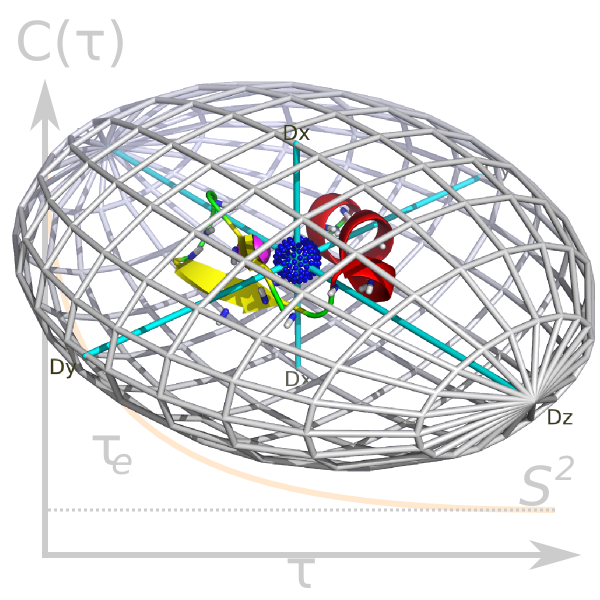
\includegraphics[width=5cm, bb=0 0 1701 1701]{graphics/analyses/model_free/model_free_600x600}
\end{figure*}


% Theory.
%%%%%%%%%

\section{Model-free theory}



% The chi-squared function.
\begin{latexonly}
    \subsection{The chi-squared function -- $\chi^2(\theta)$}
\end{latexonly}
\begin{htmlonly}
    \subsection{The chi-squared function -- $chi^2(theta)$}
\begin{htmlonly}

\index{chi-squared|textbf}

For the minimisation\index{optimisation} of the model-free models a chain of calculations, each based on a different theory, is required.
At the highest level the equation which is actually minimised is the chi-squared function
\begin{equation} \label{eq: chi-squared}
 \chi^2(\theta) = \sum_{i=1}^n \frac{(\Ri - \Ri(\theta))^2}{\sigma_i^2},
\end{equation}

\noindent where the index $i$ is the summation index ranging over all the experimentally collected relaxation data of all spins used in the analysis; $\Ri$ belongs to the relaxation data set R for an individual spin, a collection of spins, or the entire macromolecule and includes the $\Rone$, $\Rtwo$, and NOE data at all field strengths; $\Ri(\theta)$ is the back-calculated relaxation value belonging to the set R$(\theta)$; $\theta$ is the model parameter vector which when minimised is denoted by $\hat\theta$; and $\sigma_i$ is the experimental error.

The significance of the chi-squared equation~\eqref{eq: chi-squared} is that the function returns a single value which is then minimised by the optimisation algorithm to find the model-free parameter values of the given model.



% The transformed relaxation equations.
\begin{latexonly}
    \subsection{The transformed relaxation equations -- $\Ri(\theta)$}
\end{latexonly}
\begin{htmlonly}
    \subsection{The transformed relaxation equations -- R$_i(theta)$}
\end{htmlonly}

The chi-squared equation is itself dependent on the relaxation equations through the back-calculated relaxation data R$(\theta)$.
Letting the relaxation values of the set R$(\theta)$ be the $\Rone(\theta)$, $\Rtwo(\theta)$, and NOE$(\theta)$ an additional layer of abstraction can be used to simplify the calculation of the gradients and Hessians.
This involves decomposing the NOE equation into the cross relaxation rate constant $\crossrate(\theta)$ and the auto relaxation rate $\Rone(\theta)$.
Taking equation~\eqref{eq: NOE} below the transformed relaxation equations are
\begin{subequations}
\begin{align}
    \Rone(\theta) &= \Rone'(\theta), \\
    \Rtwo(\theta) &= \Rtwo'(\theta), \\
    \mathrm{NOE}(\theta)  &= 1 + \frac{\gH}{\gX} \frac{\crossrate(\theta)}{\Rone(\theta)}.
\end{align}
\end{subequations}

\noindent whereas the relaxation equations are the $\Rone(\theta)$, $\Rtwo(\theta)$, $\crossrate(\theta)$.



% The relaxation equations.
\begin{latexonly}
    \subsection{The relaxation equations -- $\Ri'(\theta)$}
\end{latexonly}
\begin{htmlonly}
    \subsection{The relaxation equations -- R$_i$ $prime(theta)$}
\end{htmlonly}

The relaxation values of the set R$'(\theta)$ include the spin-lattice\index{relaxation rate!spin-lattice}, spin-spin\index{relaxation rate!spin-spin}, and cross-relaxation rates\index{relaxation rate!cross rate} at all field strengths.
These rates are respectively \citep{Abragam61}
\begin{subequations}
\begin{align}
    \Rone(\theta) &= d \Big( J(\omega_H - \omega_X) + 3J(\omega_X) + 6J(\omega_H + \omega_X) \Big) + cJ(\omega_X),     \label{eq: R1} \\
    \Rtwo(\theta) &= \frac{d}{2} \Big( 4J(0) + J(\omega_H - \omega_X) + 3J(\omega_X) + 6J(\omega_H)                    \nonumber \\
        & \quad + 6J(\omega_H + \omega_X) \Big) + \frac{c}{6} \Big( 4J(0) + 3J(\omega_X) \Big) + R_{ex},              \label{eq: R2} \\  
    \crossrate(\theta) &= d \Big( 6J(\omega_H + \omega_X) - J(\omega_H - \omega_X) \Big),                              \label{eq: sigma_NOE}
\end{align}
\end{subequations}

\noindent where $J(\omega)$ is the power spectral density function and $R_{ex}$ is the relaxation due to chemical exchange.
The dipolar and CSA constants are defined in SI units as
\begin{gather}
 d = \frac{1}{4} \left(\frac{\mu_0}{4\pi}\right)^2 \frac{(\gH \gX \hbar)^2}{\langle r^6 \rangle}, \label{eq: dipolar constant} \\
 c = \frac{(\omega_H \Delta\sigma)^2}{3}, \label{eq: CSA constant}
\end{gather}

\noindent where $\mu_0$ is the permeability of free space, $\gH$ and $\gX$ are the gyromagnetic ratios of the $H$ and $X$ spins respectively, $\hbar$ is Plank's constant divided by $2\pi$, $r$ is the bond length, and $\Delta\sigma$ is the chemical shift anisotropy measured in ppm.
The cross-relaxation rate $\crossrate$\index{relaxation rate!cross-relaxation|textbf} is related to the steady state NOE by the equation
\begin{equation} \label{eq: NOE}
 \mathrm{NOE}(\theta) = 1 + \frac{\gH}{\gX} \frac{\crossrate(\theta)}{\Rone(\theta)}.
\end{equation}



% The spectral density functions.
\begin{latexonly}
    \subsection{The spectral density functions -- $J(\omega)$}
\end{latexonly}
\begin{htmlonly}
    \subsection{The spectral density functions -- $J(omega)$}
\end{htmlonly}

The relaxation equations are themselves dependent on the calculation of the spectral density values $J(\omega)$.
Within model-free analysis these are modelled by the original model-free formula \citep{LipariSzabo82a, LipariSzabo82b}
\begin{equation} \label{eq: J(w) model-free generic}
    J(\omega) = \frac{2}{5} \sum_{i=-k}^k c_i \cdot \tau_i \Bigg(
        \frac{S^2}{1 + (\omega \tau_i)^2}
        + \frac{(1 - S^2)(\tau_e + \tau_i)\tau_e}{(\tau_e + \tau_i)^2 + (\omega \tau_e \tau_i)^2}
    \Bigg),
\end{equation}

\noindent where $S^2$ is the square of the Lipari and Szabo generalised order parameter and $\tau_e$ is the effective correlation time.
The order parameter reflects the amplitude of the motion and the correlation time in an indication of the time scale of that motion.
The theory was extended by \citet{Clore90a} by the modelling of two independent internal motions using the equation
\begin{multline} \label{eq: J(w) model-free ext generic}
    J(\omega) = \frac{2}{5} \sum_{i=-k}^k c_i \cdot \tau_i \Bigg(
        \frac{S^2}{1 + (\omega \tau_i)^2}
        + \frac{(1 - S^2_f)(\tau_f + \tau_i)\tau_f}{(\tau_f + \tau_i)^2 + (\omega \tau_f \tau_i)^2}       \\
        + \frac{(S^2_f - S^2)(\tau_s + \tau_i)\tau_s}{(\tau_s + \tau_i)^2 + (\omega \tau_s \tau_i)^2}
    \Bigg).
\end{multline}

\noindent where $S^2_f$ and $\tau_f$ are the amplitude and timescale of the faster of the two motions whereas $S^2_s$ and $\tau_s$ are those of the slower motion.
$S^2_f$ and $S^2_s$ are related by the formula $S^2 = S^2_f \cdot S^2_s$.

If these forms of the model-free spectral density functions are unfamiliar, that is because these are the numerically stabilised forms presented in \citet{dAuvergneGooley08a}.
The original model-free spectral density functions presented in \citet{LipariSzabo82a} and \citet{Clore90a} are not the most numerically stable form of these equations.
An important problem encountered in optimisation is round-off error in which machine precision influences the result of mathematical operations.
The double reciprocal $\tau^{-1} = \tau_m^{-1} + \tau_e^{-1}$ used in the equations are operations which are particularly susceptible to round-off error, especially when $\tau_e \ll \tau_m$.
By incorporating these reciprocals into the model-free spectral density functions and then simplifying the equations this source of round-off error can be eliminated, giving relax an edge over other model-free optimisation software.


% Brownian rotational diffusion.
\subsection{Brownian rotational diffusion}

\index{diffusion!Brownian|textbf}
In equations~\eqref{eq: J(w) model-free generic} and~\eqref{eq: J(w) model-free ext generic} the generic Brownian diffusion NMR correlation function presented in \citet{dAuvergne06} has been used.
This function is
\begin{equation} \label{eq: C(tau) generic}
    C(\tau) = \frac{1}{5} \sum_{i=-k}^k c_i \cdot e^{-\tau/\tau_i},
\end{equation}

\noindent where the summation index $i$ ranges over the number of exponential terms within the correlation function.
This equation is generic in that it can describe the diffusion\index{diffusion} of an ellipsoid, a spheroid, or a sphere.



% Diffusion as an ellipsoid.
\subsubsection{Diffusion as an ellipsoid}
\index{diffusion!ellipsoid (asymmetric)|textbf}

For the ellipsoid defined by the parameter set \{$\Diff_{iso}$, $\Diff_a$, $\Diff_r$, $\alpha$, $\beta$, $\gamma$\} the variable $k$ is equal to two and therefore the index $i \in \{-2, -1, 0, 1, 2\}$.
The geometric parameters \{$\Diff_{iso}$, $\Diff_a$, $\Diff_r$\} are defined as
\begin{subequations}
\begin{align}
    & \Diff_{iso} = \tfrac{1}{3} (\Diff_x + \Diff_y + \Diff_z ),   \label{eq: Diso ellipsoid def} \\
    & \Diff_a = \Diff_z - \tfrac{1}{2}(\Diff_x + \Diff_y),         \label{eq: Da ellipsoid def} \\
    & \Diff_r = \frac{\Diff_y - \Diff_x}{2\Diff_a},                \label{eq: Dr ellipsoid def}
\end{align}
\end{subequations}

\noindent and are constrained by
\begin{subequations}
\begin{align}
    0 & < \Diff_{iso} < \infty,                                                    \label{eq: Diso lim} \\
    0 & \le \Diff_a < \frac{\Diff_{iso}}{\tfrac{1}{3} + \Diff_r} \le 3\Diff_{iso}, \label{eq: Da lim} \\
    0 & \le \Diff_r \le 1.                                                         \label{eq: Dr lim}
\end{align}
\end{subequations}

\noindent The orientational parameters \{$\alpha$, $\beta$, $\gamma$\} are the Euler angles using the z-y-z rotation notation.


The five weights $c_i$ are defined as
\begin{subequations}
\begin{align}
    c_{-2} &= \tfrac{1}{4}(d - e),     \label{eq: ellipsoid c-2} \\
    c_{-1} &= 3\delta_y^2\delta_z^2,   \label{eq: ellipsoid c-1} \\
    c_{0}  &= 3\delta_x^2\delta_z^2,   \label{eq: ellipsoid c0} \\
    c_{1}  &= 3\delta_x^2\delta_y^2,   \label{eq: ellipsoid c1} \\
    c_{2}  &= \tfrac{1}{4}(d + e),     \label{eq: ellipsoid c2}
\end{align}
\end{subequations}

\noindent where
\begin{align}
    d &= 3 \left( \delta_x^4 + \delta_y^4 + \delta_z^4 \right) - 1, \label{eq: ellipsoid d} \\
    e &= \frac{1}{\mathfrak{R}} \bigg[ (1 + 3\Diff_r) \left(\delta_x^4 + 2\delta_y^2\delta_z^2\right)
        + (1 - 3\Diff_r) \left(\delta_y^4 + 2\delta_x^2\delta_z^2\right) - 2 \left(\delta_z^4 + 2\delta_x^2\delta_y^2\right) \bigg], \label{eq: ellipsoid e}
\end{align}

\noindent and where
\begin{equation}
    \mathfrak{R} = \sqrt{1 + 3\Diff_r^2}.
\end{equation}


The five correlation times $\tau_i$ are
\begin{subequations}
\begin{align}
    1/\tau_{-2} &= 6 \Diff_{iso} - 2\Diff_a\mathfrak{R},   \label{eq: ellipsoid tau-2} \\
    1/\tau_{-1} &= 6 \Diff_{iso} - \Diff_a (1 + 3\Diff_r), \label{eq: ellipsoid tau-1} \\
    1/\tau_{0}  &= 6 \Diff_{iso} - \Diff_a (1 - 3\Diff_r), \label{eq: ellipsoid tau0} \\
    1/\tau_{1}  &= 6 \Diff_{iso} + 2\Diff_a,               \label{eq: ellipsoid tau1} \\
    1/\tau_{2}  &= 6 \Diff_{iso} + 2\Diff_a\mathfrak{R}.   \label{eq: ellipsoid tau2}
\end{align}
\end{subequations}



% Diffusion as a spheroid.
\subsubsection{Diffusion as a spheroid}
\index{diffusion!spheroid (axially symmetric)|textbf}

The variable $k$ is equal to one in the case of the spheroid\index{diffusion!spheroid (axially symmetric)|textbf} defined by the parameter set \{$\Diff_{iso}$, $\Diff_a$, $\theta$, $\phi$\}, hence $i \in \{-1, 0, 1\}$.
The geometric parameters \{$\Diff_{iso}$, $\Diff_a$\} are defined as
\begin{subequations}
\begin{align}
    & \Diff_{iso} = \tfrac{1}{3} (\Diff_\Par + 2\Diff_\Per),   \label{eq: Diso spheroid def} \\
    & \Diff_a = \Diff_\Par - \Diff_\Per.                       \label{eq: Da spheroid def}
\end{align}
\end{subequations}

\noindent and are constrained by
\begin{subequations}
\begin{gather}
    0 < \Diff_{iso} < \infty, \\
    -\tfrac{3}{2} \Diff_{iso} < \Diff_a < 3\Diff_{iso}.
\end{gather}
\end{subequations}

\noindent The orientational parameters \{$\theta$, $\phi$\} are the spherical angles defining the orientation of the major axis of the diffusion frame within the lab frame.


The three weights $c_i$ are
\begin{subequations}
\begin{align}
    c_{-1} &= \tfrac{1}{4}(3\delta_z^2 - 1)^2, \label{eq: spheroid c-1} \\
    c_{0}  &= 3\delta_z^2(1 - \delta_z^2),     \label{eq: spheroid c0} \\
    c_{1}  &= \tfrac{3}{4}(\delta_z^2 - 1)^2.  \label{eq: spheroid c1}
\end{align}
\end{subequations}

The five correlation times $\tau_i$ are
\begin{subequations}
\begin{align}
    1/\tau_{-1} &= 6\Diff_{iso} - 2\Diff_a,    \label{eq: spheroid tau-1} \\
    1/\tau_{0}  &= 6\Diff_{iso} - \Diff_a,     \label{eq: spheroid tau0} \\
    1/\tau_{1}  &= 6\Diff_{iso} + 2\Diff_a.    \label{eq: spheroid tau1}
\end{align}
\end{subequations}



% Diffusion as a sphere.
\subsubsection{Diffusion as a sphere}
\index{diffusion!sphere (isotropic)|textbf}

In the situation of a molecule diffusing as a sphere\index{diffusion!sphere (isotropic)|textbf} either described by the single parameter $\tau_m$ or $\Diff_{iso}$, the variable $k$ is equal to zero.
Therefore $i \in \{0\}$.
The single weight $c_0$ is equal to one and the single correlation time $\tau_0$ is equivalent to the global tumbling time $\tau_m$ given by
\begin{equation} \label{eq: sphere tau0}
    1/\tau_m = 6\Diff_{iso}.
\end{equation}

\noindent This is diffusion equation presented in \citet{Bloembergen48}.


% The model-free models.
%~~~~~~~~~~~~~~~~~~~~~~~

\subsection{The model-free models}

Extending the list of models given in \citet{Mandel95, Fushman97, Orekhov99b, Korzhnev01, Zhuravleva04}, the models built into relax include
\begin{latexonly}
\begin{subequations}
\renewcommand{\theequation}{\theparentequation .\arabic{equation}}
\addtocounter{equation}{-1}
\begin{align}
 m0 &= \{\},                                   \label{model: m0} \\
 m1 &= \{S^2\},                                \label{model: m1} \\
 m2 &= \{S^2, \tau_e\},                        \label{model: m2} \\
 m3 &= \{S^2, R_{ex}\},                        \label{model: m3} \\
 m4 &= \{S^2, \tau_e, R_{ex}\},                \label{model: m4} \\
 m5 &= \{S^2, S^2_f, \tau_s\},                 \label{model: m5} \\
 m6 &= \{S^2, \tau_f, S^2_f, \tau_s\},         \label{model: m6} \\
 m7 &= \{S^2, S^2_f, \tau_s, R_{ex}\},         \label{model: m7} \\
 m8 &= \{S^2, \tau_f, S^2_f, \tau_s, R_{ex}\}, \label{model: m8} \\
 m9 &= \{R_{ex}\}.                             \label{model: m9}
\end{align}
\end{subequations}
\end{latexonly}
\begin{htmlonly}
\begin{subequations}
\begin{align}
 m0 &= \{\},                                   \label{model: m0} \\
 m1 &= \{S^2\},                                \label{model: m1} \\
 m2 &= \{S^2, \tau_e\},                        \label{model: m2} \\
 m3 &= \{S^2, R_{ex}\},                        \label{model: m3} \\
 m4 &= \{S^2, \tau_e, R_{ex}\},                \label{model: m4} \\
 m5 &= \{S^2, S^2_f, \tau_s\},                 \label{model: m5} \\
 m6 &= \{S^2, \tau_f, S^2_f, \tau_s\},         \label{model: m6} \\
 m7 &= \{S^2, S^2_f, \tau_s, R_{ex}\},         \label{model: m7} \\
 m8 &= \{S^2, \tau_f, S^2_f, \tau_s, R_{ex}\}, \label{model: m8} \\
 m9 &= \{R_{ex}\}.                             \label{model: m9}
\end{align}
\end{subequations}
\end{htmlonly}

\noindent The parameter $R_{ex}$ is scaled quadratically with field strength in these models as it is assumed to be fast.
In the set theory notation, the model-free model for the spin system $i$ is represented by the symbol $\Mfset_i$.
Through the addition of the local $\tau_m$ to each of these models, only the component of Brownian rotational diffusion experienced by the spin system is probed.
These models, represented in set notation by the symbol $\Localset_i$, are
\begin{latexonly}
\begin{subequations}
\renewcommand{\theequation}{\theparentequation .\arabic{equation}}
\addtocounter{equation}{-1}
\begin{align}
 tm0 &= \{\tau_m\},                                     \label{model: tm0} \\
 tm1 &= \{\tau_m, S^2\},                                \label{model: tm1} \\
 tm2 &= \{\tau_m, S^2, \tau_e\},                        \label{model: tm2} \\
 tm3 &= \{\tau_m, S^2, R_{ex}\},                        \label{model: tm3} \\
 tm4 &= \{\tau_m, S^2, \tau_e, R_{ex}\},                \label{model: tm4} \\
 tm5 &= \{\tau_m, S^2, S^2_f, \tau_s\},                 \label{model: tm5} \\
 tm6 &= \{\tau_m, S^2, \tau_f, S^2_f, \tau_s\},         \label{model: tm6} \\
 tm7 &= \{\tau_m, S^2, S^2_f, \tau_s, R_{ex}\},         \label{model: tm7} \\
 tm8 &= \{\tau_m, S^2, \tau_f, S^2_f, \tau_s, R_{ex}\}, \label{model: tm8} \\
 tm9 &= \{\tau_m, R_{ex}\}.                             \label{model: tm9}
\end{align}
\end{subequations}
\end{latexonly}
\begin{htmlonly}
\begin{subequations}
\begin{align}
 tm0 &= \{\tau_m\},                                     \label{model: tm0} \\
 tm1 &= \{\tau_m, S^2\},                                \label{model: tm1} \\
 tm2 &= \{\tau_m, S^2, \tau_e\},                        \label{model: tm2} \\
 tm3 &= \{\tau_m, S^2, R_{ex}\},                        \label{model: tm3} \\
 tm4 &= \{\tau_m, S^2, \tau_e, R_{ex}\},                \label{model: tm4} \\
 tm5 &= \{\tau_m, S^2, S^2_f, \tau_s\},                 \label{model: tm5} \\
 tm6 &= \{\tau_m, S^2, \tau_f, S^2_f, \tau_s\},         \label{model: tm6} \\
 tm7 &= \{\tau_m, S^2, S^2_f, \tau_s, R_{ex}\},         \label{model: tm7} \\
 tm8 &= \{\tau_m, S^2, \tau_f, S^2_f, \tau_s, R_{ex}\}, \label{model: tm8} \\
 tm9 &= \{\tau_m, R_{ex}\}.                             \label{model: tm9}
\end{align}
\end{subequations}
\end{htmlonly}




% Model-free optimisation theory.
%~~~~~~~~~~~~~~~~~~~~~~~~~~~~~~~~

\subsection{Model-free optimisation theory}

The implementation of optimisation in relax is discussed in detail in Chapter~\ref{ch: optimisation}.
To understand the concepts in this subsection, it is best to look at that chapter first.


% The model-free space.
\subsubsection{The model-free space}

In model-free analysis the target function $f(\theta)$ is the chi-squared\index{chi-squared|textbf} equation
\begin{equation} \label{eq: chi2 mf}
 \chi^2(\theta) = \sum_{i=1}^n \frac{(\Ri - \Ri(\theta))^2}{\sigma_i^2},
\end{equation}

\noindent where $i$ is the summation index, $\Ri$ is the experimental relaxation data which belongs to the data set R and includes the $\Rone$, $\Rtwo$, and NOE values at all field strengths, $\Ri(\theta)$ is the back calculated relaxation data belonging to the set R$(\theta)$, and $\sigma_i$ is the experimental error.
For the optimisation of the model-free parameters while the diffusion tensor is held fixed, the summation index ranges over the relaxation data of an individual spin.
If the diffusion parameters are optimised simultaneously with the model-free parameters the summation index ranges over all relaxation data of all selected spins of the macromolecule.

Given the current parameter values the model-free function provided to the algorithm will calculate the value of the model-free spectral density function $J(\omega)$ at the five frequencies which induce NMR relaxation by using Equations~\eqref{eq: J(w) model-free generic} and \eqref{eq: J(w) model-free ext generic}.
The theoretical $\Rone$, $\Rtwo$, and NOE values are then back-calculated using Equations~\eqref{eq: R1}, \eqref{eq: R2}, \eqref{eq: sigma_NOE}, and \eqref{eq: NOE}.
Finally, the chi-squared\index{chi-squared} value is calculated using Equation~\eqref{eq: chi2 mf}.

To produce the gradient and Hessian required for model-free optimisation a large chain of first and second partial derivatives needs to be calculated.
Firstly the partial derivatives of the spectral density functions \eqref{eq: J(w) model-free generic} and \eqref{eq: J(w) model-free ext generic} are necessary.
Then the partial derivatives of the relaxation equations~\eqref{eq: R1} to~\eqref{eq: sigma_NOE} followed by the NOE equation~\eqref{eq: NOE} are needed.
Finally the partial derivative of the chi-squared\index{chi-squared} formula~\eqref{eq: chi2 mf} is required.
These first and second partial derivatives, as well as those of the components of the Brownian diffusion correlation function for non-isotropic tumbling, are presented as Chapter~\ref{ch: values, gradients, and Hessians}.


% Grid search.
\subsubsection{Grid search}

Due to the complexity of the curvature of the model-free space, the grid point with the lowest chi-squared\index{chi-squared} value may in fact be on the opposite side of the space to the local minimum.
Therefore the model-free space renders many optimisation algorithms ineffective \citep{dAuvergneGooley08a}.


% Constraints.
\subsubsection{Parameter constraints}

To understand this section, please see Section~\ref{sect: constraint algorithms} on page~\pageref{sect: constraint algorithms}.
For model-free analysis, linear constraints are the most useful type of constraint as the correlation time $\tau_f$ can be restricted to being less than $\tau_s$ by using the inequality $\tau_s - \tau_f \geqslant 0$.

For the parameters specific to individual spins the linear constraints in the notation of \eqref{eq: linear constraint} are
\begin{equation}
    \begin{pmatrix}
        1 & 0 & 0 & 0 & 0 & 0 & 0 & 0 & 0 \\
        1 & 0 & 0 & 0 & 0 & 0 & 0 & 0 & 0 \\
        0 & 1 & 0 & 0 & 0 & 0 & 0 & 0 & 0 \\
        0 &-1 & 0 & 0 & 0 & 0 & 0 & 0 & 0 \\
        0 & 0 & 1 & 0 & 0 & 0 & 0 & 0 & 0 \\
        0 & 0 &-1 & 0 & 0 & 0 & 0 & 0 & 0 \\
        1 & 1 & 0 & 0 & 0 & 0 & 0 & 0 & 0 \\
        1 & 0 & 1 & 0 & 0 & 0 & 0 & 0 & 0 \\
        0 & 0 & 0 & 1 & 0 & 0 & 0 & 0 & 0 \\
        0 & 0 & 0 & 0 & 1 & 0 & 0 & 0 & 0 \\
        0 & 0 & 0 & 0 & 0 & 1 & 0 & 0 & 0 \\
        0 & 0 & 0 & 0 &-1 & 1 & 0 & 0 & 0 \\
        0 & 0 & 0 & 0 & 0 & 0 & 1 & 0 & 0 \\
        0 & 0 & 0 & 0 & 0 & 0 & 0 & 1 & 0 \\
        0 & 0 & 0 & 0 & 0 & 0 & 0 &-1 & 0 \\
        0 & 0 & 0 & 0 & 0 & 0 & 0 & 0 & 1 \\
        0 & 0 & 0 & 0 & 0 & 0 & 0 & 0 &-1 \\
    \end{pmatrix}
    \cdot
    \begin{pmatrix}
        S^2 \\
        S^2_f \\
        S^2_s \\
        \tau_e \\
        \tau_f \\
        \tau_s \\
        R_{ex} \\
         r \\
        CSA \\
    \end{pmatrix}
    \geqslant
    \begin{pmatrix}
        0 \\
        -1 \\
        0 \\
        -1 \\
        0 \\
        -1 \\
        0 \\
        0 \\
        0 \\
        0 \\
        0 \\
        0 \\
        0 \\
        0.9e^{-10} \\
        2e^{-10} \\
        300e^{-6} \\
        0 \\
    \end{pmatrix}.
\end{equation}

\noindent  Through the isolation of each individual element, the constraints can be seen to be equivalent to
\begin{subequations}
\begin{gather} 
    0 \leqslant S^2 \leqslant 1, \\
    0 \leqslant S^2_f \leqslant 1, \\
    0 \leqslant S^2_s \leqslant 1, \\
    S^2 \leqslant S^2_f, \\
    S^2 \leqslant S^2_s, \\
    \tau_e \geqslant 0, \\
    \tau_f \geqslant 0, \\
    \tau_s \geqslant 0, \\
    \tau_s \geqslant 0, \\
    \tau_f \leqslant \tau_s, \\
    R_{ex} \geqslant 0, \\
    0.9e^{-10} \leqslant r \leqslant 2e^{-10}, \\
    -300e^{-6} \leqslant CSA \leqslant 0.
\end{gather} 
\end{subequations}

To prevent the computationally expensive optimisation of failed models in which the internal correlation times minimise to infinity \citep{dAuvergneGooley06}, the constraint $\tau_e, \tau_f, \tau_s \leqslant 2\tau_m$ was implemented.
When the global correlation time is fixed the constraints in the matrix notation of \eqref{eq: linear constraint} are
\begin{equation}
    \begin{pmatrix}
        -1 &  0 &  0 \\
         0 & -1 &  0 \\
         0 &  0 & -1 \\
    \end{pmatrix}
    \cdot
    \begin{pmatrix}
        \tau_e \\
        \tau_f \\
        \tau_s \\
    \end{pmatrix}
    \geqslant
    \begin{pmatrix}
        -2\tau_m \\
        -2\tau_m \\
        -2\tau_m \\
    \end{pmatrix}.
\end{equation}

\noindent  However when the global correlation time $\tau_m$ is one of the parameters being optimised the constraints become
\begin{equation}
    \begin{pmatrix}
        2 & -1 &  0 &  0 \\
        2 &  0 & -1 &  0 \\
        2 &  0 &  0 & -1 \\
    \end{pmatrix}
    \cdot
    \begin{pmatrix}
        \tau_m \\
        \tau_e \\
        \tau_f \\
        \tau_s \\
    \end{pmatrix}
    \geqslant
    \begin{pmatrix}
        0 \\
        0 \\
        0 \\
    \end{pmatrix}.
\end{equation}

For the parameters of the diffusion tensor the constraints utilised are
\begin{subequations}
\begin{gather} 
    0 \leqslant \tau_m \leqslant 200.0e^{-9}, \\
    \Diff_a \geqslant 0, \\
    0 \leqslant \Diff_r \leqslant 1,
\end{gather} 
\end{subequations}

\noindent  which in the matrix notation of \eqref{eq: linear constraint} become
\begin{equation}
    \begin{pmatrix}
         1 &  0 &  0 \\
        -1 &  0 &  0 \\
         0 &  1 &  0 \\
         0 &  0 &  1 \\
         0 &  0 & -1 \\
    \end{pmatrix}
    \cdot
    \begin{pmatrix}
        \tau_m \\
        \Diff_a \\
        \Diff_r \\
    \end{pmatrix}
    \geqslant
    \begin{pmatrix}
        0 \\
        -200.0e^{-9} \\
        0 \\
        0 \\
        -1 \\
    \end{pmatrix}.
\end{equation}

\noindent  The upper limit of 200~ns on $\tau_m$ prevents the parameter from heading towards infinity when model failure occurs (see \citet{dAuvergneGooley06}).
This can significantly decrease the computation time.
To isolate the prolate spheroid\index{diffusion!spheroid (axially symmetric)} the constraint
\begin{equation}
    \begin{pmatrix}
         1 \\
    \end{pmatrix}
    \cdot
    \begin{pmatrix}
        \Diff_a \\
    \end{pmatrix}
    \geqslant
    \begin{pmatrix}
        0 \\
    \end{pmatrix},
\end{equation}

\noindent is used whereas to isolate the oblate spheroid\index{diffusion!spheroid (axially symmetric)} the constraint used is
\begin{equation}
    \begin{pmatrix}
         -1 \\
    \end{pmatrix}
    \cdot
    \begin{pmatrix}
        \Diff_a \\
    \end{pmatrix}
    \geqslant
    \begin{pmatrix}
        0 \\
    \end{pmatrix}.
\end{equation}

Dependent on the model optimised, the matrix $A$ and vector $b$ are constructed from combinations of the above linear constraints.


% Diagonal scaling.
\subsubsection{Diagonal scaling}

The concept of diagonal scaling is explained in Section~\ref{sect: diagonal scaling} on page~\pageref{sect: diagonal scaling}.

For the model-free analysis the scaling factor of one is used for the order parameter and a scaling factor of $1e^{-12}$ is used for the correlation times.
The $R_{ex}$ parameter is scaled to be the chemical exchange rate of the first field strength.
The scaling matrix for the parameters \{$S^2$, $S^2_f$, $S^2_s$, $\tau_e$, $\tau_f$, $\tau_s$, $R_{ex}$, $r$, $CSA$\} of individual spins is
\begin{equation}
    \begin{pmatrix}
        1 &  0 &  0 &  0 &  0 &  0 &  0 &  0 &  0 \\
        0 &  1 &  0 &  0 &  0 &  0 &  0 &  0 &  0 \\
        0 &  0 &  1 &  0 &  0 &  0 &  0 &  0 &  0 \\
        0 &  0 &  0 &  1e^{-12} &  0 &  0 &  0 &  0 &  0 \\
        0 &  0 &  0 &  0 &  1e^{-12} &  0 &  0 &  0 &  0 \\
        0 &  0 &  0 &  0 &  0 &  1e^{-12} &  0 &  0 &  0 \\
        0 &  0 &  0 &  0 &  0 &  0 &  (2\pi \omega_H)^{-2} &  0 &  0 \\
        0 &  0 &  0 &  0 &  0 &  0 &  0 &  1e^{-10} &  0 \\
        0 &  0 &  0 &  0 &  0 &  0 &  0 &  0 &  1e^{-4} \\
    \end{pmatrix}.
\end{equation}

\noindent  For the ellipsoidal\index{diffusion!ellipsoid (asymmetric)} diffusion parameters \{$\tau_m$, $\Diff_a$, $\Diff_r$, $\alpha$, $\beta$, $\gamma$\} the scaling matrix is
\begin{equation}
    \begin{pmatrix}
        1e^{-12} &  0 &  0 &  0 &  0 &  0 \\
        0 &  1e^7 &  0 &  0 &  0 &  0 \\
        0 &  0 &  1 &  0 &  0 &  0 \\
        0 &  0 &  0 &  1 &  0 &  0 \\
        0 &  0 &  0 &  0 &  1 &  0 \\
        0 &  0 &  0 &  0 &  0 &  1 \\
    \end{pmatrix}.
\end{equation}

\noindent  For the spheroidal\index{diffusion!spheroid (axially symmetric)} diffusion parameters \{$\tau_m$, $\Diff_a$, $\theta$, $\phi$\} the scaling matrix is
\begin{equation}
    \begin{pmatrix}
        1e^{-12} &  0 &  0 &  0 \\
        0 &  1e^7 &  0 &  0 \\
        0 &  0 &  1 &  0 \\
        0 &  0 &  0 &  1 \\
    \end{pmatrix}.
\end{equation}




% Optimisation of a single model-free model.
%%%%%%%%%%%%%%%%%%%%%%%%%%%%%%%%%%%%%%%%%%%%

\section{Optimisation of a single model-free model}\label{sect: single mf model}


% The sample script.
%~~~~~~~~~~~~~~~~~~~

\subsection{Single model-free model script mode -- the sample script}

The sample script which demonstrates the optimisation of model-free model $m4$ which consists of the parameters \{$S^2$, $\tau_e$, $R_{ex}$\} is \file{model\osus{}free\ossep{}single\osus{}model.py}.
The text of the script is:

\begin{lstlisting}
# Script for model-free analysis.

# Create the data pipe.
name = 'm4'
pipe.create(name, 'mf')

# Set up the 15N spins.
sequence.read('noe.500.out', res_num_col=1, res_name_col=2)
spin.name('N')
spin.element(element='N', spin_id='@N')
spin.isotope('15N', spin_id='@N')

# Load the relaxation data.
relax_data.read(ri_id='R1_600',  ri_type='R1',  frq=600.0*1e6, file='r1.600.out',  res_num_col=1, data_col=3, error_col=4)
relax_data.read(ri_id='R2_600',  ri_type='R2',  frq=600.0*1e6, file='r2.600.out',  res_num_col=1, data_col=3, error_col=4)
relax_data.read(ri_id='NOE_600', ri_type='NOE', frq=600.0*1e6, file='noe.600.out', res_num_col=1, data_col=3, error_col=4)
relax_data.read(ri_id='R1_500',  ri_type='R1',  frq=500.0*1e6, file='r1.500.out',  res_num_col=1, data_col=3, error_col=4)
relax_data.read(ri_id='R2_500',  ri_type='R2',  frq=500.0*1e6, file='r2.500.out',  res_num_col=1, data_col=3, error_col=4)
relax_data.read(ri_id='NOE_500', ri_type='NOE', frq=500.0*1e6, file='noe.500.out', res_num_col=1, data_col=3, error_col=4)

# Initialise the diffusion tensor.
diffusion_tensor.init(10e-9, fixed=True)

# Create all attached protons.
sequence.attach_protons()

# Define the magnetic dipole-dipole relaxation interaction.
interatom.define(spinid1='@N', spin_id2='@H', direct_bond=True)
interatom.set_dist(spin_id1='@N', spin_id2='@H', ave_dist=1.02 * 1e-10)
#interatom.unit_vectors()

# Define the CSA relaxation interaction.
value.set(-172 * 1e-6, 'csa')

# Select the model-free model.
model_free.select_model(model=name)

# Grid search.
minimise.grid_search(inc=11)

# Minimise.
minimise.execute('newton')

# Monte Carlo simulations.
monte_carlo.setup(number=100)
monte_carlo.create_data()
monte_carlo.initial_values()
minimise.execute('newton')
eliminate()
monte_carlo.error_analysis()

# Finish.
results.write(file='results', force=True)
state.save('save', force=True)
\end{lstlisting}


% The explanation.
%~~~~~~~~~~~~~~~~~

\subsection{Single model-free model script mode -- explanation}

The above script consists of three major sections:
\begin{description}
  \item[Loading of data] Firstly a data pipe called \promptstring{m4} is created to hold all of the analysis data.
    Then the $^{15}$N spin system data consisting of molecule, residue, and spin information is loaded into relax from the columns of the \file{noe.500.out} file, assuming that only residue numbers and names are present and are in the first and second columns respectively.
    The options of this \uf{sequence\ufsep{}read} user function allow the molecule name, residue number, residue name, spin number, or spin name columns to be specified if desired.
    The $^{15}$N spin is then set up using the \uf{spin} user functions.
    The next part is to load all of the relaxation data, to set up the initial diffusion tensor, create the $^1$H spins required for the magnetic dipole-dipole interaction, and to set up the magnetic dipole-dipole and CSA relaxation mechanisms.
    Finally the model-free model \promptstring{m4} is chosen.
  \item[Optimisation] The optimisation of model-free models requires an initial grid search to find a position close to the minimum, followed by the high precision Newton optimisation together with the Method of Multipliers constraint algorithm \citep{dAuvergneGooley08a}.
    Errors are propagated from the relaxation data to the model-free parameters via Monte Carlo simulations which is a multi-step process in relax (designed for flexibility and to teach how the simulations are constructed and carried out).
  \item[Data output] The last stage consists of writing out the XML formatted results file which contains all of the data in the current data pipe, as well as the XML formatted save file which contains not only the current data pipe data but all of the relax data store data.
    Both files can be loaded back into relax later on.
\end{description}



% Optimisation of all model-free models.
%%%%%%%%%%%%%%%%%%%%%%%%%%%%%%%%%%%%%%%%

\section{Optimisation of all model-free models}


% The sample script.
%~~~~~~~~~~~~~~~~~~~

\subsection{All model-free models script mode -- the sample script}

The sample script which demonstrates the optimisation of all model-free models from $m0$ to $m9$ of individual spins is \file{model\osus{}free\ossep{}mf\osus{}multimodel.py}.
The important parts of the script are:

\begin{lstlisting}
# Set the data pipe names (also the names of preset model-free models).
pipes = ['m0', 'm1', 'm2', 'm3', 'm4', 'm5', 'm6', 'm7', 'm8', 'm9']

# Loop over the pipes.
for name in pipes:
    # Create the data pipe.
    pipe.create(name, 'mf')
    
    # Set up the 15N spins.
    sequence.read('noe.500.out', res_num_col=1)
    spin.name('N')
    spin.element(element='N', spin_id='@N')
    spin.isotope('15N', spin_id='@N')
    
    # Load a PDB file.
    structure.read_pdb('example.pdb')
    
    # Load the relaxation data.
    relax_data.read(ri_id='R1_600',  ri_type='R1',  frq=600.0*1e6, file='r1.600.out',  res_num_col=1, data_col=3, error_col=4)
    relax_data.read(ri_id='R2_600',  ri_type='R2',  frq=600.0*1e6, file='r2.600.out',  res_num_col=1, data_col=3, error_col=4)
    relax_data.read(ri_id='NOE_600', ri_type='NOE', frq=600.0*1e6, file='noe.600.out', res_num_col=1, data_col=3, error_col=4)
    relax_data.read(ri_id='R1_500',  ri_type='R1',  frq=500.0*1e6, file='r1.500.out',  res_num_col=1, data_col=3, error_col=4)
    relax_data.read(ri_id='R2_500',  ri_type='R2',  frq=500.0*1e6, file='r2.500.out',  res_num_col=1, data_col=3, error_col=4)
    relax_data.read(ri_id='NOE_500', ri_type='NOE', frq=500.0*1e6, file='noe.500.out', res_num_col=1, data_col=3, error_col=4)
    
    # Set up the diffusion tensor.
    diffusion_tensor.init(1e-8, fixed=True)
    
    # Generate the 1H spins for the magnetic dipole-dipole relaxation interaction.
    sequence.attach_protons()
    
    # Define the magnetic dipole-dipole relaxation interaction.
    interatom.define(spin_id1='@N', spin_id2='@H', direct_bond=True)
    interatom.set_dist(spin_id1='@N', spin_id2='@H', ave_dist=1.02 * 1e-10)
    structure.get_pos('@N')
    structure.get_pos('@H')
    interatom.unit_vectors()
    
    # Define the chemical shift relaxation interaction.
    value.set(-172 * 1e-6, 'csa', spin_id='@N')
    
    # Select the model-free model.
    model_free.select_model(model=name)
    
    # Minimise.
    minimise.grid_search(inc=11)
    minimise.execute('newton')
    
    # Write the results.
    results.write(file='results', force=True)

# Save the program state.
state.save('save', force=True)
\end{lstlisting}


% The explanation.
%~~~~~~~~~~~~~~~~~

\subsection{All model-free models script mode -- explanation}

The above script is very similar in spirit to the previous single model script in section~\ref{sect: single mf model} on page~\pageref{sect: single mf model}.
The major difference is that this script loops over all of the model-free models, saving all of the results in the \file{save.bz2} file.



% Model-free model selection.
%%%%%%%%%%%%%%%%%%%%%%%%%%%%%

\section{Model-free model selection}


% The sample script.
%~~~~~~~~~~~~~~~~~~~

\subsection{Model-free model selection script mode -- the sample script}

The sample script which demonstrates both model-free model elimination and model-free model selection between models from $m0$ to $m9$ is \file{model\osus{}free\ossep{}modsel.py}.
The text of the script is:

\begin{lstlisting}
# Set the data pipe names.
pipes = ['m0', 'm1', 'm2', 'm3', 'm4', 'm5', 'm6', 'm7', 'm8', 'm9']

# Loop over the data pipe names.
for name in pipes:
    print("\n\n# " + name + " #")
    
    # Create the data pipe.
    pipe.create(name, 'mf')
    
    # Reload precalculated results from the file 'm1/results', etc.
    results.read(file='results', dir=name)

# Model elimination.
eliminate()

# Model selection.
model_selection(method='AIC', modsel_pipe='aic')

# Write the results.
state.save('save', force=True)
results.write(file='results', force=True)
\end{lstlisting}


% The explanation.
%~~~~~~~~~~~~~~~~~

\subsection{Model-free model selection script mode -- explanation}

This script is designed to be used in conjunction with the \file{model\osus{}free\ossep{}mf\osus{}multimodel.py} script in the previous section.
It will load all of the results files from the previous script and then perform the following:
\begin{description}
  \item[Model-free model elimination]  The optimisation of model-free models performed by the previous script will fail for certain data sets together with certain models.
    To ensure that these models are never selected, they are removed from the analysis (see \citet{dAuvergneGooley06}).
  \item[Model-free model selection]  The AIC model selection as described in \citet{dAuvergneGooley03} will be used to determine which model-free model best describes the relaxation data.
  \item[Data output]  Finally both a save state and result file will be created.
\end{description}

These three sample scripts describe the basic components of model-free analysis.
However a full analysis requires the construction of a much more complex iterative procedure.
The following sections will describe both the original diffusion seeded approaches as well as the new model-free protocol built into relax.


% The methodology of Mandel et al., 1995.
%%%%%%%%%%%%%%%%%%%%%%%%%%%%%%%%%%%%%%%%%

\section{The methodology of Mandel et al., 1995}
\label{sect: Mandel 1995}

% Mandel et al., 1995 figure.
\begin{figure}
  \centerline{
    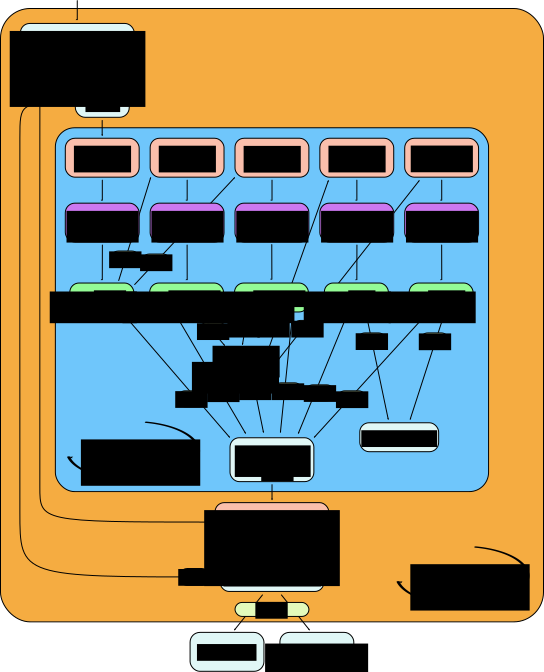
\includegraphics[
      width=0.8\textwidth,
      bb=0 0 436 539
    ]
    {images/model_free/mandel95}
  }
  \caption[A schematic of the model-free optimisation protocol of Mandel et al., 1995]{
    A schematic of the model-free optimisation protocol of \citet{Mandel95}.
    This specific protocol is for single field strength data.
    The initial diffusion tensor estimate is calculated using the $\Rtwo/\Rone$ ratio.
    The diffusion parameters of $\Diffset$ are held constant while model-free models $m1$ to $m5$ (\ref{model: m1}--\ref{model: m5}) of the set $\Mfset_i$ for each spin $i$ are optimised and 500 Monte Carlo simulations executed.
    Using a web of ANOVA statistical tests, specifically $\chi^2$ and F-tests, a step-up hypothesis testing model selection procedure is used to choose the best model-free model.
    These steps are repeated for all spins of the molecule.
    The global model $\Space$, the union of $\Diffset$ and all $\Mfset_i$, is then optimised.
    These steps are repeated until convergence of the global model.
    The iterative process is repeated for both isotropic diffusion (sphere) and anisotropic diffusion (spheroid).
  }
  \label{fig: Mandel et al.}
\end{figure}

By presenting a systematic methodology for obtaining a consistent model-free description of the dynamics of the system, the manuscript of \citet{Mandel95} revolutionised the application of model-free analysis.
The full protocol is presented in Figure~\ref{fig: Mandel et al.}.

All of the data analysis techniques required for this protocol can be implemented within relax.
The chi-squared distributions required for the chi-squared tests are constructed by Modelfree4 from the Monte Carlo simulations.
If the optimisation algorithms and Monte Carlo simulations built into relax are utilised, then the relax script will need to construct the chi-squared distributions from the results as this is not yet coded into relax.
The specific step-up hypothesis testing model selection of \citet{Mandel95} is available through the \uf{model\ufus{}selection} user function.
Coding the rest of the protocol into a script should be straightforward.

To implement this analysis, a number of scripts would need to be written.
There is no sample script in relax for performing this analysis.
The simple sample scripts from above would need to be extended.
For example a starting script for determining the initial diffusion tensor estimates based on the R1/R2 ratio of \citet{Kay89} would have to be written.
The tensor from this script could then be feed into the \file{model\osus{}free\ossep{}mf\osus{}multimodel.py} script, followed by the \file{model\osus{}free\ossep{}modsel.py} script, and then a third script written to optimise the diffusion tensor.
A master script could be written first run the initial diffusion tensor script, then to iteratively execute the last three scripts until convergence, and finally to select the best diffusion model (see Figure~\ref{fig: Mandel et al.}).
Alternatively, these could all be combined into one super script.



% The diffusion seeded paradigm.
%%%%%%%%%%%%%%%%%%%%%%%%%%%%%%%%

\section{The diffusion seeded paradigm}
\label{sect: diffusion seeded paradigm}

Ever since the original Lipari and Szabo papers \citep{LipariSzabo82a, LipariSzabo82b}, the question of how to obtain the model-free description of the system has followed the route in which the diffusion tensor is initially estimated.
Using this rough estimate, the model-free models are optimised for each spin system $i$, the best model selected, and then the global model $\Space$ of the diffusion model $\Diffset$ with each model-free model $\Mfset_i$ is optimised.
This procedure is then repeated using the diffusion tensor parameters of $\Space$ as the initial input.
Finally the global model is selected.
The full protocol, when combined with AIC model selection \citep{dAuvergneGooley03}, is illustrated in Figure~\ref{fig: init diff estimate}.


% The diffusion seeded paradigm figure.
\begin{figure}
  \centerline{
    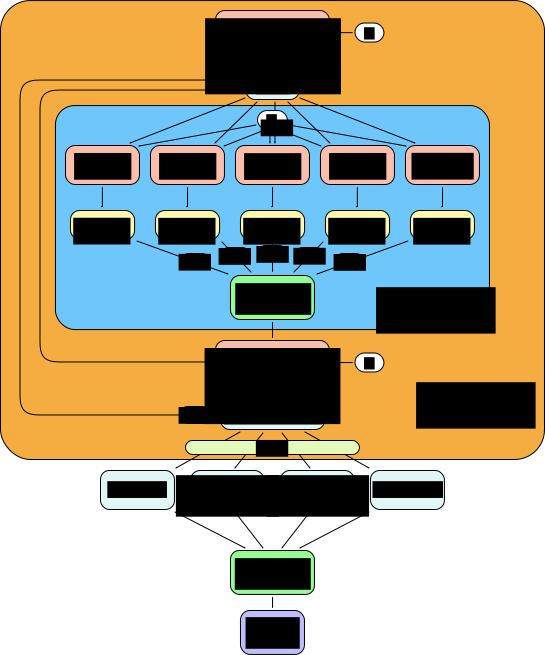
\includegraphics[
      width=0.8\textwidth,
      bb=0 0 437 523
    ]
    {images/model_free/init_diff_est}
  }
  \caption[Model-free analysis using the diffusion seeded paradigm]{
    A schematic of model-free analysis using the diffusion seeded paradigm -- the initial diffusion tensor estimate -- together with AIC model selection and model elimination.
    The initial estimates of the parameters of $\Diffset$ are held constant while model-free models $m0$ to $m9$ (\ref{model: m0}--\ref{model: m9}) of the set $\Mfset_i$ for each spin system $i$ are optimised, model elimination applied to remove failed models, and AIC model selection used to determine the best model.
    The global model $\Space$, the union of $\Diffset$ and all $\Mfset_i$, is then optimised.
    These steps are repeated until convergence of the global model.
    The entire iterative process is repeated for each of the Brownian diffusion models.
    Finally AIC model selection is used to determine the best description of the dynamics of the molecule by selecting between the global models $\Space$ including the sphere, oblate spheroid, prolate spheroid, and ellipsoid.
    Once the solution has been found, Monte Carlo simulations can be utilised for error analysis.
  }
  \label{fig: init diff estimate}
\end{figure}

Again this protocol is not implemented in the relax sample scripts.
This would have to be implemented in exactly the same manner as described in the previous section, but using the AIC model selection build into relax.
Constructing this set of scripts, or a single master script, would be much easier than the \citet{Mandel95} protocol as Modelfree4 would not need to be used, and the handling of F-tests and chi-squared tests is avoided.



% The new model-free optimisations protocol.
%%%%%%%%%%%%%%%%%%%%%%%%%%%%%%%%%%%%%%%%%%%%

\section{The new model-free optimisation protocol}
\label{sect: new model-free protocol}

Here a new, fully automated model-free optimisation protocol will be presented.
This protocol, defined in \citet{dAuvergneGooley07} and \citet{dAuvergneGooley08b}, is significantly different from all those that came before, reversing the diffusion seeded paradigm as detailed below.
Within relax it is referred to as the ``new protocol'' or the ``d'Auvergne protocol''.
The later name is to allow for more advanced protocols to be developed and added to relax by adventurous users in the future.
Note that for advanced model-free analysis protocols, such as this one, that multiple field relaxation data is essential.


% The model-free models.
%~~~~~~~~~~~~~~~~~~~~~~~

\subsection{The new protocol -- model-free models}

The study of the dynamics of a macromolecule using model-free analysis to interpret the $\Rone$ and $\Rtwo$ relaxation rates together with the steady-state heteronuclear NOE brings two distinct, yet linked physical theories into play.
The Brownian rotational diffusion of the molecule is the major contributor to relaxation.
Although having less of an influence on relaxation the internal dynamics of individual nuclei within the molecule is nevertheless significant.
The model-free description of the internal motion and the global diffusion of the entire molecule are theories which are linked due to their dependence on the same relaxation data.
The model-free models for individual spin system constructed from the original and extended model-free theories \citep{LipariSzabo82a, LipariSzabo82b, Clore90a} are assembled using parametric restrictions, the dropping of insignificant parameters, and the addition of the chemical exchange parameter $R_{ex}$.
Labelled as $m0$ to $m9$ (Models~\ref{model: m0}--\ref{model: m9} on page \pageref{model: m9}) these models are an extended list of those in \citep{Fushman97, Orekhov99b, Korzhnev01, Zhuravleva04}.



% The diffusion tensor.
%~~~~~~~~~~~~~~~~~~~~~~

\subsection{The new protocol -- the diffusion tensor}


% The ellipsoid.
\subsubsection{The ellipsoid}
\index{diffusion!ellipsoid (asymmetric)|textbf}

The most general form of Brownian rotational diffusion of macromolecules is the diffusion of an ellipsoid, a diffusion also labelled as asymmetric or fully anisotropic.
This diffusion tensor can be fully specified by the geometric parameters $\Diff_x$, $\Diff_y$, and $\Diff_z$, the eigenvalues of the tensor, as well as three orientational parameters, the Euler angles\index{Euler angles} $\alpha$, $\beta$, and $\gamma$.
The diffusion equation for an ellipsoid was derived using the reasoning of \citet{Einstein05} in the two papers of \citet{Perrin34} and \citet{Perrin36}.
Following this, \citet{Favro60} unknowingly derived the same equations as presented in \citet{Perrin36} using a pseudo quantum mechanical approach.
Borrowing heavily from \citet{Perrin36}, \citet{Woessner62} derived the correlation function relevant for NMR relaxation of a bond vector rigidly attached to an ellipsoid.
However these equations are not fully simplified and the parameter set \{$\Diff_x$, $\Diff_y$, $\Diff_z$, $\alpha$, $\beta$, $\gamma$\}, the eigenvalues and Euler angles\index{Euler angles} defining the tensor, is not optimally constructed for minimisation.
A parameter shift to the set \{$\Diff_{iso}$, $\Diff_a$, $\Diff_r$, $\alpha$, $\beta$, $\gamma$\}, whereby the three geometric parameters are respectively the isotropic, anisotropic, and rhombic components of the diffusion tensor, drastically simplifies optimisation and is how the diffusion tensor is implemented within relax.


% The spheroid.
\subsubsection{The spheroid}
\index{diffusion!spheroid (axially symmetric)|textbf}

When two of the eigenvalues of the diffusion tensor are equal the molecule diffuses as a spheroid.
This is also called axially symmetric anisotropic diffusion and can be described by the two geometric parameters $\Diff_{iso}$ and $\Diff_a$ together with the polar angle $\theta$ and azimuthal angle $\phi$ which define the unique axis of the diffusion tensor.
Two classes of spheroid can be distinguished dependent on the relative values of the eigenvalues -- the prolate and oblate spheroids.
By using parametric constraints, both tensor types can be optimised within relax.


% The sphere.
\subsubsection{The sphere}
\index{diffusion!sphere (isotropic)|textbf}

The simplest form of diffusion occurs when all three eigenvalues are equal and the molecule diffuses as a sphere.
This isotropic rotation can be characterised by the single parameter $\Diff_{iso}$ which is related to the global correlation time by the formula $1/\tau_m = 6\Diff_{iso}$ \citep{Bloembergen48}.


% The local tm model-free models.
\begin{latexonly}
    \subsubsection{The local $\tau_m$ model-free models}
\end{latexonly}
\begin{htmlonly}
    \subsubsection{The local $tau_m$ model-free models}
\end{htmlonly}

Not only can the diffusion tensor be optimised as a global model affecting all spins of the molecule but a set of model-free models can be constructed in which each spin is assumed to diffuse independently.
In these models a single local $\tau_m$ parameter approximates the true, multiexponential description of the Brownian rotational diffusion of the molecule.
Each spin of the macromolecule is treated independently.
Another set of model-free models which include the local $\tau_m$ parameter can be created and include $tm0$ to $tm9$ (Models~\ref{model: tm0}--\ref{model: tm9} on page \pageref{model: tm0}).
These are simply models $m0$ to $m9$ with the local $\tau_m$ parameter added.
These models are an extension of the ideas introduced in \citet{Barbato92} and \citet{Schurr94} whereby the model $tm2$, the original Lipari and Szabo model-free equation with a local $\tau_m$ parameter, is optimised to avoid issues with inaccurate diffusion tensor approximations.


% Determination of the diffusion tensor from the local tm parameter.
\begin{latexonly}
    \subsubsection{Determination of the diffusion tensor from the local $\tau_m$ parameter}
\end{latexonly}
\begin{htmlonly}
    \subsubsection{Determination of the diffusion tensor from the local $tau_m$ parameter}
\end{htmlonly}

In \citet{Bruschweiler95} and further investigated in \citet{Lee97}, a methodology for determining the diffusion tensor from the local $\tau_m$ parameter together with the orientation of the XH bond represented by the unit vector $\mu_i$ was presented.
A local $\tau_m$ value was obtained for each spin $i$ by optimising model $tm2$.
The $\tau_{m,i}$ values were approximated using the quadric model
\begin{equation} \label{eq: quadric}
 (6 \tau_{m,i})^{-1} = \mu_i^T Q \mu_i,
\end{equation}

\noindent where the eigenvalues of the matrix $Q$ are defined as $Q_x = (\Diff_y + \Diff_z)/2$, $Q_y = (\Diff_x + \Diff_z)/2$, and $Q_z = (\Diff_x + \Diff_y)/2$.
The diffusion tensor is then found by linear least-squares fitting.



% The universal solution.
%~~~~~~~~~~~~~~~~~~~~~~~~

\begin{latexonly}
    \subsection{The universal solution $\Univset$}
\end{latexonly}
\begin{htmlonly}
    \subsection{The universal solution $U$}
\end{htmlonly}
\label{sect: universal solution}

The complex model-free problem, in which the motions of each spin are both mathematically and statistically dependent on the diffusion tensor and vice versa, was formulated using set theory in \citet{dAuvergneGooley07}.
This paper is important for understanding the entire concept of the new protocol in relax and for truly grasping the complexity of the model-free problem.
The solution $\widehat{\Univset}$ to the model-free problem was derived as an element of the universal set $\Univset$, the union of the diverse model-free parameter spaces $\Space$.
Each set $\Space$ was constructed from the union of the model-free models $\Mfset$ for all spins and the diffusion parameter set $\Diffset$.
A single parameter loss on a single spin shifts optimisation to a different space $\Space$.
Ever since the seminal work of \citet{Kay89} the model-free problem has been tackled by first finding an initial estimate of the diffusion tensor and then determining the model-free dynamics of the system (see Sections~\ref{sect: Mandel 1995} on page~\pageref{sect: Mandel 1995} and~\ref{sect: diffusion seeded paradigm} on page~\pageref{sect: diffusion seeded paradigm}).
This diffusion seeded paradigm is now highly evolved and much theory has emerged to improve this path to the solution $\widehat{\Univset}$.
The technique can, at times, suffer from a number of issues including the two minima problem of the spheroid diffusion tensor parameter space, the appearance of artificial chemical exchange \citep{Tjandra96}, the appearance of artificial nanosecond motions \citep{Schurr94}, and the hiding of internal nanosecond motions caused by the violation of the rigidity assumption \citep{Orekhov95b, Orekhov99b, Orekhov99a}.



% Model-free analysis in reverse.
%~~~~~~~~~~~~~~~~~~~~~~~~~~~~~~~~

\subsection{Model-free analysis in reverse}

% New model-free optimisation protocol figure.
\begin{figure}
  \centerline{
    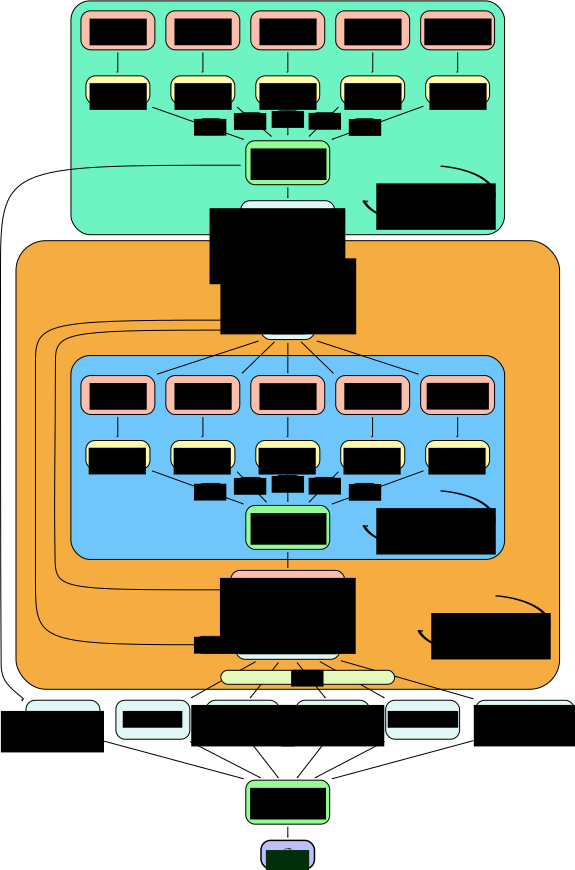
\includegraphics[
      width=0.8\textwidth,
      bb=0 0 461 697
    ]
    {images/model_free/new_protocol}
  }
  \caption[A schematic of the new model-free optimisation protocol]{
    A schematic of the new model-free optimisation protocol.
    Initially models $tm0$ to $tm9$ (\ref{model: tm0}--\ref{model: tm9}) of the set $\Localset_i$ for each spin system $i$ are optimised, model elimination used to remove failed models, and AIC model selection used to pick the best model.
    Once all the $\Localset_i$ have been determined for the system the the local $\tau_m$ parameter is removed, the model-free parameters are held fixed, and the global diffusion parameters of $\Diffset$ are optimised.
    These parameters are used as input for the central part of the schematic which follows the same procedure as that of Figure~\ref{fig: init diff estimate}.
    Convergence is however precisely defined as identical models $\Space$, identical $\chi^2$ values, and identical parameters $\theta$ between two iterations.
    The universal solution $\widehat{\Univset}$, the best description of the dynamics of the molecule, is determined using AIC model selection to select between the local $\tau_m$ models for all spins, the sphere, oblate spheroid, prolate spheroid, ellipsoid, and possibly hybrid models whereby multiple diffusion tensors have been applied to different parts of the molecule.
  }
  \label{fig: new protocol}
\end{figure}


A different approach was proposed in \citet{dAuvergneGooley08b} for finding the universal solution $\widehat{\Univset}$ of the extremely complex, convoluted model-free optimisation and modelling problem \citep{dAuvergneGooley07}, defined as
\begin{equation} \label{eq: universal solution}
 \widehat{\Univset} = \hat\theta \in \left\{ \Space: \min_{\hat\theta \in \Univset} \KL(\hat\theta) \right\},
  \text{\quad s.t. }
  \hat\theta = \arg \min \left\{\chi^2(\theta): \theta \in \Space \right\}.
\end{equation}

\noindent This notation says that the minimised parameter vector within the space $\Space$ which minimises the common Kullback-Leibler discrepancy\index{discrepancy!Kullback-Leibler} $\KL$ is selected from the universal set $\Univset$ as the universal solution $\widehat{\Univset}$.
The discrepancy of \citet{KullbackLeibler51} is a measure of how well the model fits the data, in this case how well the global model $\Space$ of the diffusion tensor together with the model-free models of all residues fits the relaxation data.
This selection is subject to the condition that $\hat\theta$ is the argument or specific parameter vector which minimises the chi-squared\index{chi-squared} function $\chi^2(\theta)$ such that $\theta$ is an element of the space $\Space$.
Whereas the minimisation of the continuous chi-squared\index{chi-squared} function within the single space $\Space$ belongs to the mathematical field of optimisation \citep{NocedalWright99}, the selection of the universe $\Space$ which minimises the discrepancy\index{discrepancy} belongs to the statistical field of model selection \citep{Akaike73,Schwarz78,LinhartZucchini86,Zucchini00,dAuvergneGooley03}.

This new model-free optimisation protocol incorporates the ideas of the local $\tau_m$ model-free model \citep{Barbato92, Schurr94} and the optimisation of the diffusion tensor using information from these models, analogously to the linear least-squares fitting of the quadric model \citep{Bruschweiler95, Lee97}.
The protocol also follows the lead of the model-free optimisation protocol presented in \citet{Butterwick04} whereby the diffusion seeded paradigm was reversed.
Rather than starting with an initial estimation of the global diffusion tensor from the set $\Diffset$ the protocol starts with the model-free parameters from $\Mfset$.

The first step of the \citet{Butterwick04} protocol is the reduced spectral density mapping of \citet{Farrow95}.
As $R_{ex}$ has been eliminated from the analysis, three model-free models corresponding to $tm1$, $tm2$, and $tm5$ (Models~\ref{model: tm1}, \ref{model: tm2}, and \ref{model: tm5} on page~\pageref{model: tm1}) are employed.
The model-free parameters are optimised using the reduced spectral density values and the best model is selected using F-tests.
The spherical, spheroidal, and ellipsoidal diffusion tensors are obtained by linear least-squares fitting of the quadric model of Equation~\eqref{eq: quadric} using the local $\tau_m$ values \citep{Bruschweiler95, Lee97}.
The best diffusion model is selected via F-tests and refined by iterative elimination of spins systems with high chi-squared values.
This tensor is used to calculate local $\tau_m$ values for each spin system, approximating the multiexponential sum of the Brownian rotational diffusion correlation function with a single exponential, using the quadric model of Equation~\eqref{eq: quadric}.
In the final step of the protocol these $\tau_m$ values are fixed and $m1$, $m2$, and $m5$ (Models~\ref{model: m1}, \ref{model: m2}, and \ref{model: m5} on page~\pageref{model: m1}) are optimised and the best model-free model selected using F-tests.

The new model-free protocol built into relax utilises the core foundation of the \citet{Butterwick04} protocol yet its divergent implementation is designed to solve the universal equation of \citet{dAuvergneGooley07} to find $\widehat{\Univset}$ (Equation~\ref{eq: universal solution}).
Models $tm0$ to $tm9$ (\ref{model: tm0}--\ref{model: tm9} on page \pageref{model: tm0}) in which no global diffusion parameters exist are employed to significantly collapse the complexity of the problem.
Model-free minimisation \citep{dAuvergneGooley08a}, model elimination \citep{dAuvergneGooley06}, and then AIC\index{model selection!AIC} model selection \citep{Akaike73, dAuvergneGooley03} can be carried out in the absence of the influence of global parameters.
By removing the local $\tau_m$ parameter and holding the model-free parameter values constant these models can then be used to optimise the diffusion parameters of $\Diffset$.
Model-free optimisation, model elimination, AIC model selection, and optimisation of the global model $\Space$ is iterated until convergence.
The iterations allow for sliding between different universes $\Space$ to enable the collapse of model complexity, to refine the diffusion tensor, and to find the solution within the universal set $\Univset$.
The last step is the AIC model selection between the different diffusion models.
Because the AIC criterion approximates the Kullback-Leibler discrepancy \citep{KullbackLeibler51}, central to the universal solution of Equation~\eqref{eq: universal solution}, it was chosen for all three model selection steps over BIC model selection \citep{Schwarz78, dAuvergneGooley03, Chen04}.
The new protocol avoids the problem of under-fitting\index{under-fitting} whereby artificial motions appear, avoids the problems involved in finding the initial diffusion tensor within $\Diffset$, and avoids the problem of hidden internal nanosecond motions and the inability to slide between universes to get to $\widehat{\Univset}$ (see \citet{dAuvergneGooley07} for more details).
The full protocol is summarised in Figure~\ref{fig: new protocol}.


% Script UI.
%%%%%%%%%%%%

\newpage
\section{The new protocol in the prompt/script UI mode}


% The sample script.
%~~~~~~~~~~~~~~~~~~~

\subsection{d'Auvergne protocol script mode -- the sample script}

The sample script for performing this new analysis is \file{sample\osus{}scripts\ossep{}model\osus{}free\ossep{}dauvergne\osus{}protocol\linebreak[0]{}.py}.
The full script is replicated below.
The docstring at the start of the script explains the practical implementation of the full protocol.
If your copy of the \file{dauvergne\osus{}protocol.py} script taken from the same relax version as this manual does not match the text below, please contact the relax developers via the relax-devel mailing list\index{mailing list!relax-devel} (see section~\ref{sect: relax-devel mailing list} on page~\pageref{sect: relax-devel mailing list}).
To use this script, copy it to a dedicated directory containing your PDB file and relaxation data files.
The protocol will produce many files and directories, so it is best that these are placed within a dedicated and results directory.
The contents of the script are:

\begin{lstlisting}
"""Script for black-box model-free analysis.

This script is designed for those who appreciate black-boxes or those who appreciate complex code.  Importantly data at multiple magnetic field strengths is essential for this analysis.  The script will need to be heavily tailored to the molecule in question by changing the variables just below this documentation.  If you would like to change how model-free analysis is performed, the code in the class Main can be changed as needed.  For a description of object-oriented coding in python using classes, functions/methods, self, etc., see the python tutorial.

If you have obtained this script without the program relax, please visit http://www.nmr-relax.com.


References
==========

The model-free optimisation methodology herein is that of:

    d'Auvergne, E. J. and Gooley, P. R. (2008b). Optimisation of NMR dynamic models II. A new methodology for the dual optimisation of the model-free parameters and the Brownian rotational diffusion tensor. J. Biomol. NMR, 40(2), 121-133

Other references for features of this script include model-free model selection using Akaike's Information Criterion:

    d'Auvergne, E. J. and Gooley, P. R. (2003). The use of model selection in the model-free analysis of protein dynamics. J. Biomol. NMR, 25(1), 25-39.

The elimination of failed model-free models and Monte Carlo simulations:

    d'Auvergne, E. J. and Gooley, P. R. (2006). Model-free model elimination: A new step in the model-free dynamic analysis of NMR relaxation data. J. Biomol. NMR, 35(2), 117-135.

Significant model-free optimisation improvements:

    d'Auvergne, E. J. and Gooley, P. R. (2008a). Optimisation of NMR dynamic models I. Minimisation algorithms and their performance within the model-free and Brownian rotational diffusion spaces. J. Biomol. NMR, 40(2), 107-109.

Rather than searching for the lowest chi-squared value, this script searches for the model with the lowest AIC criterion.  This complex multi-universe, multi-dimensional search is formulated using set theory as the universal solution:

    d'Auvergne, E. J. and Gooley, P. R. (2007). Set theory formulation of the model-free problem and the diffusion seeded model-free paradigm. 3(7), 483-494.

The basic three references for the original and extended model-free theories are:

    Lipari, G. and Szabo, A. (1982a). Model-free approach to the interpretation of nuclear magnetic-resonance relaxation in macromolecules I. Theory and range of validity. J. Am. Chem. Soc., 104(17), 4546-4559.

    Lipari, G. and Szabo, A. (1982b). Model-free approach to the interpretation of nuclear magnetic-resonance relaxation in macromolecules II. Analysis of experimental results. J. Am. Chem. Soc., 104(17), 4559-4570.

    Clore, G. M., Szabo, A., Bax, A., Kay, L. E., Driscoll, P. C., and Gronenborn, A.M. (1990). Deviations from the simple 2-parameter model-free approach to the interpretation of N-15 nuclear magnetic-relaxation of proteins. J. Am. Chem. Soc., 112(12), 4989-4991.


How to use this script
======================

The value of the variable DIFF_MODEL will determine the behaviour of this script.  The five diffusion models used in this script are:

    Model I   (MI)   - Local tm.
    Model II  (MII)  - Sphere.
    Model III (MIII) - Prolate spheroid.
    Model IV  (MIV)  - Oblate spheroid.
    Model V   (MV)   - Ellipsoid.

Model I must be optimised prior to any of the other diffusion models, while the Models II to V can be optimised in any order.  To select the various models, set the variable DIFF_MODEL to the following strings:

    MI   - 'local_tm'
    MII  - 'sphere'
    MIII - 'prolate'
    MIV  - 'oblate'
    MV   - 'ellipsoid'

This approach has the advantage of eliminating the need for an initial estimate of a global diffusion tensor and removing all the problems associated with the initial estimate.

It is important that the number of parameters in a model does not exceed the number of relaxation data sets for that spin.  If this is the case, the list of models in the MF_MODELS and LOCAL_TM_MODELS variables will need to be trimmed.


Model I - Local tm
~~~~~~~~~~~~~~~~~~

This will optimise the diffusion model whereby all spin of the molecule have a local tm value, i.e. there is no global diffusion tensor.  This model needs to be optimised prior to optimising any of the other diffusion models.  Each spin is fitted to the multiple model-free models separately, where the parameter tm is included in each model.

AIC model selection is used to select the models for each spin.


Model II - Sphere
~~~~~~~~~~~~~~~~~

This will optimise the isotropic diffusion model.  Multiple steps are required, an initial optimisation of the diffusion tensor, followed by a repetitive optimisation until convergence of the diffusion tensor.  Each of these steps requires this script to be rerun. For the initial optimisation, which will be placed in the directory './sphere/init/', the following steps are used:

The model-free models and parameter values for each spin are set to those of diffusion model MI.

The local tm parameter is removed from the models.

The model-free parameters are fixed and a global spherical diffusion tensor is minimised.


For the repetitive optimisation, each minimisation is named from 'round_1' onwards.  The initial 'round_1' optimisation will extract the diffusion tensor from the results file in './sphere/init/', and the results will be placed in the directory './sphere/round_1/'.  Each successive round will take the diffusion tensor from the previous round.  The following steps are used:

The global diffusion tensor is fixed and the multiple model-free models are fitted to each spin.

AIC model selection is used to select the models for each spin.

All model-free and diffusion parameters are allowed to vary and a global optimisation of all parameters is carried out.


Model III - Prolate spheroid
~~~~~~~~~~~~~~~~~~~~~~~~~~~~

The methods used are identical to those of diffusion model MII, except that an axially symmetric diffusion tensor with Da >= 0 is used.  The base directory containing all the results is './prolate/'.


Model IV - Oblate spheroid
~~~~~~~~~~~~~~~~~~~~~~~~~~

The methods used are identical to those of diffusion model MII, except that an axially symmetric diffusion tensor with Da <= 0 is used.  The base directory containing all the results is './oblate/'.


Model V - Ellipsoid
~~~~~~~~~~~~~~~~~~~

The methods used are identical to those of diffusion model MII, except that a fully anisotropic diffusion tensor is used (also known as rhombic or asymmetric diffusion).  The base directory is './ellipsoid/'.



Final run
~~~~~~~~~

Once all the diffusion models have converged, the final run can be executed.  This is done by setting the variable DIFF_MODEL to 'final'.  This consists of two steps, diffusion tensor model selection, and Monte Carlo simulations.  Firstly AIC model selection is used to select between the diffusion tensor models.  Monte Carlo simulations are then run solely on this selected diffusion model.  Minimisation of the model is bypassed as it is assumed that the model is already fully optimised (if this is not the case the final run is not yet appropriate).

The final black-box model-free results will be placed in the file 'final/results'.
"""

# Python module imports.
from time import asctime, localtime

# relax module imports.
from auto_analyses.dauvergne_protocol import dAuvergne_protocol


# Analysis variables.
#####################

# The diffusion model.
DIFF_MODEL = 'local_tm'

# The model-free models.  Do not change these unless absolutely necessary, the protocol is likely to fail if these are changed.
MF_MODELS = ['m0', 'm1', 'm2', 'm3', 'm4', 'm5', 'm6', 'm7', 'm8', 'm9']
LOCAL_TM_MODELS = ['tm0', 'tm1', 'tm2', 'tm3', 'tm4', 'tm5', 'tm6', 'tm7', 'tm8', 'tm9']

# The grid search size (the number of increments per dimension).
GRID_INC = 11

# The optimisation technique.
MIN_ALGOR = 'newton'

# The number of Monte Carlo simulations to be used for error analysis at the end of the analysis.
MC_NUM = 500

# Automatic looping over all rounds until convergence (must be a boolean value of True or False).
CONV_LOOP = True



# Set up the data pipe.
#######################

# The following sequence of user function calls can be changed as needed.

# Create the data pipe.
pipe_bundle = "mf (%s)" % asctime(localtime())
name = "origin - " + pipe_bundle
pipe.create(name, 'mf', bundle=pipe_bundle)

# Load the PDB file.
structure.read_pdb('1f3y.pdb', set_mol_name='Ap4Aase', read_model=3)

# Set up the 15N and 1H spins (both backbone and Trp indole sidechains).
structure.load_spins('@N', ave_pos=True)
structure.load_spins('@NE1', ave_pos=True)
structure.load_spins('@H', ave_pos=True)
structure.load_spins('@HE1', ave_pos=True)
spin.isotope('15N', spin_id='@N*')
spin.isotope('1H', spin_id='@H*')

# Set up the 15N spins (alternative to the structure-based approach).
#sequence.read(file='noe.500.out', dir=None, mol_name_col=1, res_num_col=2, res_name_col=3, spin_num_col=4, spin_name_col=5)
#spin.element(element='N', spin_id='@N*')
#spin.isotope('15N', spin_id='@N*')

# Generate the 1H spins for the magnetic dipole-dipole relaxation interaction (alternative to the structure-based approach).
#sequence.attach_protons()

# Load the relaxation data.
relax_data.read(ri_id='R1_600',  ri_type='R1',  frq=599.719*1e6, file='r1.600.out',  mol_name_col=1, res_num_col=2, res_name_col=3, spin_num_col=4, spin_name_col=5, data_col=6, error_col=7)
relax_data.read(ri_id='R2_600',  ri_type='R2',  frq=599.719*1e6, file='r2.600.out',  mol_name_col=1, res_num_col=2, res_name_col=3, spin_num_col=4, spin_name_col=5, data_col=6, error_col=7)
relax_data.read(ri_id='NOE_600', ri_type='NOE', frq=599.719*1e6, file='noe.600.out', mol_name_col=1, res_num_col=2, res_name_col=3, spin_num_col=4, spin_name_col=5, data_col=6, error_col=7)
relax_data.read(ri_id='R1_500',  ri_type='R1',  frq=500.208*1e6, file='r1.500.out',  mol_name_col=1, res_num_col=2, res_name_col=3, spin_num_col=4, spin_name_col=5, data_col=6, error_col=7)
relax_data.read(ri_id='R2_500',  ri_type='R2',  frq=500.208*1e6, file='r2.500.out',  mol_name_col=1, res_num_col=2, res_name_col=3, spin_num_col=4, spin_name_col=5, data_col=6, error_col=7)
relax_data.read(ri_id='NOE_500', ri_type='NOE', frq=500.208*1e6, file='noe.500.out', mol_name_col=1, res_num_col=2, res_name_col=3, spin_num_col=4, spin_name_col=5, data_col=6, error_col=7)

# Deselect spins to be excluded (including unresolved and specifically excluded spins).
deselect.read(file='unresolved', dir=None, spin_id_col=None, mol_name_col=1, res_num_col=2, res_name_col=3, spin_num_col=4, spin_name_col=5, sep=None, spin_id=None, boolean='AND', change_all=False)
deselect.read(file='exclude', spin_id_col=1)

# Define the magnetic dipole-dipole relaxation interaction.
interatom.define(spin_id1='@N', spin_id2='@H', direct_bond=True)
interatom.define(spin_id1='@NE1', spin_id2='@HE1', direct_bond=True)
interatom.set_dist(spin_id1='@N*', spin_id2='@H*', ave_dist=1.02 * 1e-10)
interatom.unit_vectors()

# Define the chemical shift relaxation interaction.
value.set(-172 * 1e-6, 'csa', spin_id='@N*')



# Execution.
############

# Do not change!
dAuvergne_protocol(pipe_name=name, pipe_bundle=pipe_bundle, diff_model=DIFF_MODEL, mf_models=MF_MODELS, local_tm_models=LOCAL_TM_MODELS, grid_inc=GRID_INC, min_algor=MIN_ALGOR, mc_sim_num=MC_NUM, conv_loop=CONV_LOOP)
\end{lstlisting}


% The analysis variables.
%~~~~~~~~~~~~~~~~~~~~~~~~

\subsection{d'Auvergne protocol script mode -- analysis variables} \label{sect: d'Auvergne protocol script variables}

At the start of the script you will notice a number of \pycode{Analysis variables}.
Unless you know what you are doing, you should only change the \pycode{DIFF\_MODEL} variable to the following:
\begin{description}
  \item[\pystring{local\_tm}:]  This is the first diffusion model which must be optimised prior to optimising any of the other diffusion models.
    It consists of the local $\tau_m$ models (equations~\ref{model: tm0} to~\ref{model: tm9} on page~\pageref{model: tm0}).
  \item[\pystring{sphere}:]  This second diffusion model is that of isotropic Brownian diffusion.
  \item[\pystring{prolate}:]  This third diffusion model is that of the prolate axially-symmetric rotor.
  \item[\pystring{oblate}:]  This fourth diffusion model is that of the oblate axially-symmetric rotor.
  \item[\pystring{ellipsoid}:]  This fifth diffusion model is that of fully rhombic Brownian diffusion (see \citet{Perrin34,Perrin36} for the original theory).
  \item[\pystring{final}:]  This is a special value which will finalise the analysis by selecting the best diffusion model to describe your system and to perform Monte Carlo simulations for error propagation.
\end{description}

The \pycode{MF\_MODELS} and  \pycode{LOCAL\_TM\_MODELS} variables specify which model-free models will be used in the analysis.
But, as the full protocol behind this script which is designed to find the solution of the universal set $\Univset$ (see section~\ref{sect: universal solution} on page~\pageref{sect: universal solution}) expects that all these models are present, you should not change these variables.
If you do remove some model-free models, you should fully expect to see artificial motions which you will not be able to distinguish from the real molecular motions.

The next variables \pycode{GRID\_INC} and \pycode{MIN\_ALGOR} are related to the optimisation of the model-free models.
These should also not be touched unless you fully understand the consequences (and have read \citet{dAuvergneGooley08a}).
The variable \pycode{MC\_NUM} specifies the number of Monte Carlo simulations.
This number can be increased but, for realistic parameter errors in your publication, it should not set lower than 500 simulations.

Finally the \pycode{CONV\_LOOP} variable is designed to make your life easier.
If left at the value of \pycode{True}, the script will iterate until convergence (see Figure~2 in \citet{dAuvergneGooley08b} to understand this concept).
If changed to \pycode{False}, then you will need to run the script manually for the 15 or so iterations of each diffusion model, and then repeat this for all diffusion models II to V.


% Initialisation of the data pipe.
%~~~~~~~~~~~~~~~~~~~~~~~~~~~~~~~~~

\subsection{d'Auvergne protocol script mode -- data pipe initialisation}

The next part of the script between the \pycode{Analysis variables} and execution sets up a data pipe with all of the spin information and relaxation data to pass into the automated protocol.
The data pipe is created in the lines:

\begin{lstlisting}[firstnumber=156]
# Create the data pipe.
pipe_bundle = "mf (%s)" % asctime(localtime())
name = "origin - " + pipe_bundle
pipe.create(name, 'mf', bundle=pipe_bundle)
\end{lstlisting}

Firstly a data pipe bundle name is created containing the date and time at the point the script is first executed.
This pipe bundle is used to group together all of the data pipes created automatically by the protocol.
See section~\ref{sect: data pipe bundles} on page~\pageref{sect: data pipe bundles} for more details.

The data pipe name used for this initial setup is set to \pycode{origin - mf (x)} where \pycode{x} is the data and time again.
This name is unique and will not clash with the data pipes created within the protocol.
The \uf{pipe\ufsep{}create} command will create the data pipe and add it to a new pipe bundle.


% Spin systems.
%~~~~~~~~~~~~~~

\subsection{d'Auvergne protocol script mode -- setting up the spin systems}

To see how to set up the spin system data in all possible situations, please see Chapter~\ref{ch: data model} for a thorough description.
Here two different methods are presented.
The first is by extracting the spins from a PDB file which is first loaded with:

\begin{lstlisting}[firstnumber=161]
# Load the PDB file.
structure.read_pdb('1f3y.pdb', set_mol_name='Ap4Aase', read_model=3)
\end{lstlisting}
\index{PDB}

This will read the \nth{3} model from the 1F3Y PDB file and name the single molecule as \pystring{Ap4Aase}.
The $^{15}$N and $^1$H spins for the backbone and tryptophan indole sidechain are extracted from the structure with the user functions:

\begin{lstlisting}[firstnumber=164]
# Set up the 15N and 1H spins (both backbone and Trp indole sidechains).
structure.load_spins('@N', ave_pos=True)
structure.load_spins('@NE1', ave_pos=True)
structure.load_spins('@H', ave_pos=True)
structure.load_spins('@HE1', ave_pos=True)
\end{lstlisting}

As the PDB file does not contain isotope information, this is set with the user functions:

\begin{lstlisting}[firstnumber=169]
spin.isotope('15N', spin_id='@N*')
spin.isotope('1H', spin_id='@H*')
\end{lstlisting}

The spin ID \pystring{@N*} uses regular expression and will match both the \pystring{N} and \pystring{NE1} spins.

The alternative approach is if a structure is missing.
This is the commented out code:

\begin{lstlisting}[firstnumber=172]
# Set up the 15N spins (alternative to the structure-based approach).
sequence.read(file='noe.500.out', dir=None, mol_name_col=1, res_num_col=2, res_name_col=3, spin_num_col=4, spin_name_col=5)
spin.element(element='N', spin_id='@N*')
spin.isotope('15N', spin_id='@N*')

# Generate the 1H spins for the magnetic dipole-dipole relaxation interaction (alternative to the structure-based approach).
sequence.attach_protons()
\end{lstlisting}

To use this, you will need to place comments (the \pycode{\#} character) in front of the previous \uf{structure\ufsep{}read\ufus{}pdb}, \uf{structure\ufsep{}load\ufus{}spins} and \uf{spin\ufsep{}isotope} user functions.
Then uncomment the \uf{sequence\ufsep{}read}, \uf{spin\ufsep{}element}, \uf{spin\ufsep{}isotope} and \uf{sequence\ufsep{}attach\ufus{}protons} user functions.
The $^{15}$N spins will be extracted from the \file{noe.500.out} file.
The \uf{spin\ufsep{}element} and \uf{spin\ufsep{}isotope} user functions set the information required for relax to understand which relaxation mechanisms are active.
Finally the \uf{sequence\ufsep{}attach\ufus{}protons} user function will automatically attach protons to all nitrogen spin systems.
As this method is devoid of atomic positional information, the N-H bonds are absent and the diffusion models requiring structural information (the spheroids and ellipsoid) must be skipped.


% Loading the data.
%~~~~~~~~~~~~~~~~~~

\subsection{d'Auvergne protocol script mode -- loading the data}

The next step is to load the relaxation data for each spin system.
The sample script assumes that the NOE, $\Rone$ and $\Rtwo$ data was generated using relax.
One of the six user function calls is:

\begin{lstlisting}[firstnumber=180]
# Load the relaxation data.
relax_data.read(ri_id='R1_600',  ri_type='R1',  frq=599.719*1e6, file='r1.600.out',  mol_name_col=1, res_num_col=2, res_name_col=3, spin_num_col=4, spin_name_col=5, data_col=6, error_col=7)
\end{lstlisting}

This pattern is repeated for all of the relaxation data files loaded.
The important points are that each relaxation data set must have its own unique identification string (\pycode{ri\_id}), the relaxation data type specified (\pycode{ri\_type}) and the frequency in Hertz (not MHz) specified.
Note that the frequency must be the exact value -- see the \pycode{sfrq} parameter in the Varian \file{procpar} file or the \pycode{SFO1} parameter in the Bruker \file{acqus} file.


% Deselection.
%~~~~~~~~~~~~~

\subsection{d'Auvergne protocol script mode -- deselection}

The sample script now presents the deselection of spins using two different files:

\begin{lstlisting}[firstnumber=188]
# Deselect spins to be excluded (including unresolved and specifically excluded spins).
deselect.read(file='unresolved', dir=None, spin_id_col=None, mol_name_col=1, res_num_col=2, res_name_col=3, spin_num_col=4, spin_name_col=5, sep=None, spin_id=None, boolean='AND', change_all=False)
deselect.read(file='exclude', spin_id_col=1)
\end{lstlisting}

The \file{unresolved} file contains a list of spins which are unresolved in all spectra.
If relax has been used for calculating the NOE and fitting the relaxation curves, then this step is not needed as the relaxation data files will not have any data for the spins deselected in those analyses.
The second file \file{exclude} is a list of spin ID strings (see section~\ref{sect: spin ID} on page~\pageref{sect: spin ID}) of spins that for which ever reason are to be excluded from the analysis.


% The relaxation interactions.
%~~~~~~~~~~~~~~~~~~~~~~~~~~~~~

\subsection{d'Auvergne protocol script mode -- relaxation interactions}

The next step is to fully specify all of the relaxation interactions active on the spins of interest.
Firstly the magnetic dipole-dipole interaction is defined between directly bonded nitrogens and protons:

\begin{lstlisting}[firstnumber=192]
# Define the magnetic dipole-dipole relaxation interaction.
interatom.define(spin_id1='@N', spin_id2='@H', direct_bond=True)
interatom.define(spin_id1='@NE1', spin_id2='@HE1', direct_bond=True)
interatom.set_dist(spin_id1='@N*', spin_id2='@H*', ave_dist=1.02 * 1e-10)
interatom.unit_vectors()
\end{lstlisting}

The regular expression \pystring{@N*} and \pystring{@H*} cannot be used with the \uf{dipole\ufus{}pair\ufsep{}} define user function as otherwise \prompt{@N} spins will be connected to \prompt{@HE1} spins of the same tryptophan residue and \prompt{@H} spins to \prompt{@NE1} spins.
The average interatomic distance is set to 1.02 \AA ngstrom (though the \uf{dipole\ufus{}pair\ufsep{}set\ufus{}dist} user function expects the units of meters).
The \uf{dipole\ufus{}pair\ufsep{}unit\ufus{}vectors} is used to calculate the averaged unit vector between the two atoms.

Secondly the chemical shift anisotropy (CSA) relaxation mechanism is defined via the single command:

\begin{lstlisting}[firstnumber=198]
# Define the chemical shift relaxation interaction.
value.set(-172 * 1e-6, 'csa', spin_id='@N*')
\end{lstlisting}

If your system does not experience CSA relaxation, the value can be set to zero.


% Execution.
%~~~~~~~~~~~
\subsection{d'Auvergne protocol script mode -- execution}

Once the data is set up and you have modified your script to match your analysis needs, then the data pipe, pipe bundle and analysis variables are passed into the \module{dAuvergne\pyus{}protocol} class.
This is the final line of the script:

\begin{lstlisting}[firstnumber=203]
# Execution.
############

# Do not change!
dAuvergne_protocol(pipe_name=name, pipe_bundle=pipe_bundle, diff_model=DIFF_MODEL, mf_models=MF_MODELS, local_tm_models=LOCAL_TM_MODELS, grid_inc=GRID_INC, min_algor=MIN_ALGOR, mc_sim_num=MC_NUM, conv_loop=CONV_LOOP)
\end{lstlisting}

This script needs to be executed multiple times, once for each of the diffusion models.
For example if the \pycode{DIFF\_MODEL} variable is set to \pystring{ellipsoid}, you can run relax with:

\example{\$ relax --tee log.ellipsoid dauvergne\_protocol.py}

You should use a different log file for each diffusion model, though relax will prevent you from overwriting an old log file.
Note that the \file{log.*} files for each diffusion model may end up being a few gigabytes in size.

For a full analysis of a protein system, the analysis may require between one to two weeks to complete.
This can be speed up using Gary Thompson's multi-processor code (see section~\ref{sect: multi-processor} on page~\pageref{sect: multi-processor}).
The analysis is performed as described in the previous sections and summarised in Figure~\ref{fig: new protocol}.
If you are curious, the implementation is within a very large relax script called \file{auto\osus{}analyses\ossep{}dauvergne\osus{}protocol.py} (which must never be changed).
This automatic analysis script hides all of the complexity of the full protocol from the sample script.



% d'Auvergne protocol in the GUI.
%%%%%%%%%%%%%%%%%%%%%%%%%%%%%%%%%

\newpage
\section{The new protocol in the GUI}

A model-free analysis can be performed within the GUI (see Figure~\ref{fig: screenshot: model-free analysis} on page~\pageref{fig: screenshot: model-free analysis}).
This analysis is that of the fully automated d'Auvergne protocol which can be chosen via the analysis selection wizard (Figure~\ref{fig: screenshot: analysis wizard} on page~\pageref{fig: screenshot: analysis wizard}).
Please see Section~\ref{sect: new model-free protocol} on page~\pageref{sect: new model-free protocol} for a description of this new model-free protocol.
As mentioned previously, please note that this protocol requires multiple field relaxation data.

The GUI is designed to be robust -- you should be able to set up all the input data and parameters in any order with relax returning you warnings if something is missing.
The analysis will only execute once everything is correctly set up.
If this is not the case, clicking on the \guibutton{Execute relax} button will display a warning window explaining what the issue is rather than initialising the analysis.
Despite the self-explanatory nature of the GUI a tutorial on how to use the GUI, with screenshots, will be presented below.

If the \gui{Protocol mode} field is left to the \gui{Fully automated} setting then, after clicking on \guibutton{Execute relax}, the calculation can be left to complete.
It is highly recommended to check the log messages in the relax controller window, at least at the start of the analysis, to make sure that all the data is being read correctly and everything is set up as desired.
All warnings should be carefully checked as these can indicate a fatal problem.
If you would like to log all the messages into a file, relax can be run with:

\example{\$ relax -g --log log}

Note that the size of this \file{log} file could end up being in the gigabyte range for a model-free analysis.

For the full analysis to complete, for a protein system this may take about a week.
Depending on the nature of the problem and the speed of the computer, the calculation time may be significantly shorter or longer.
To speed up the calculations, if you have access to multiple cores and/or hyper-threading, the GUI can be run using Gary Thompson's multi-processor framework (see section~\ref{sect: multi-processor} on page~\pageref{sect: multi-processor}).
For example on a dual-core, dual-CPU system, four calculations can be run simultaneously.
In this case, the GUI can be launched with:

\example{\$ mpirun -np 5 /usr/local/bin/relax --multi=`mpi4py' --gui --log log}

This assumes that OpenMPI and the Python mpi4py module have been installed on your system, and relax is installed into the \directory{\ossep{}usr\ossep{}local\ossep{}bin\ossep{}} directory.
If this is successful, you should only see a single relax GUI window (and not five windows) and in the relax controller, you should see text similar to:

\example{Processor fabric:  MPI 2.1 running via mpi4py with 4 slave processors \& 1 master.  Using Open MPI 1.4.3.}

If you are using a different MPI implementation, please see the documentation of that implementation to see how to launch a program in MPI mode.
Finally as the calculation takes so long, we will run the calculations at a lower priority so that the computer is not slowed down too much and remains responsive.
Therefore this model-free GUI analysis tutorial will be launched with the full command:

\example{\$ nice -n 15 mpirun -np 5 /usr/local/bin/relax --multi=`mpi4py' --gui --log log}


% Initialisation of the data pipe.
%~~~~~~~~~~~~~~~~~~~~~~~~~~~~~~~~~

\subsection{d'Auvergne protocol GUI mode -- data pipe initialisation}

First launch the analysis selection wizard (see Figure~\ref{fig: screenshot: analysis wizard} on page \pageref{fig: screenshot: analysis wizard}) and click on the model-free analysis button.

\begin{minipage}[h]{\linewidth}
  \centerline{
    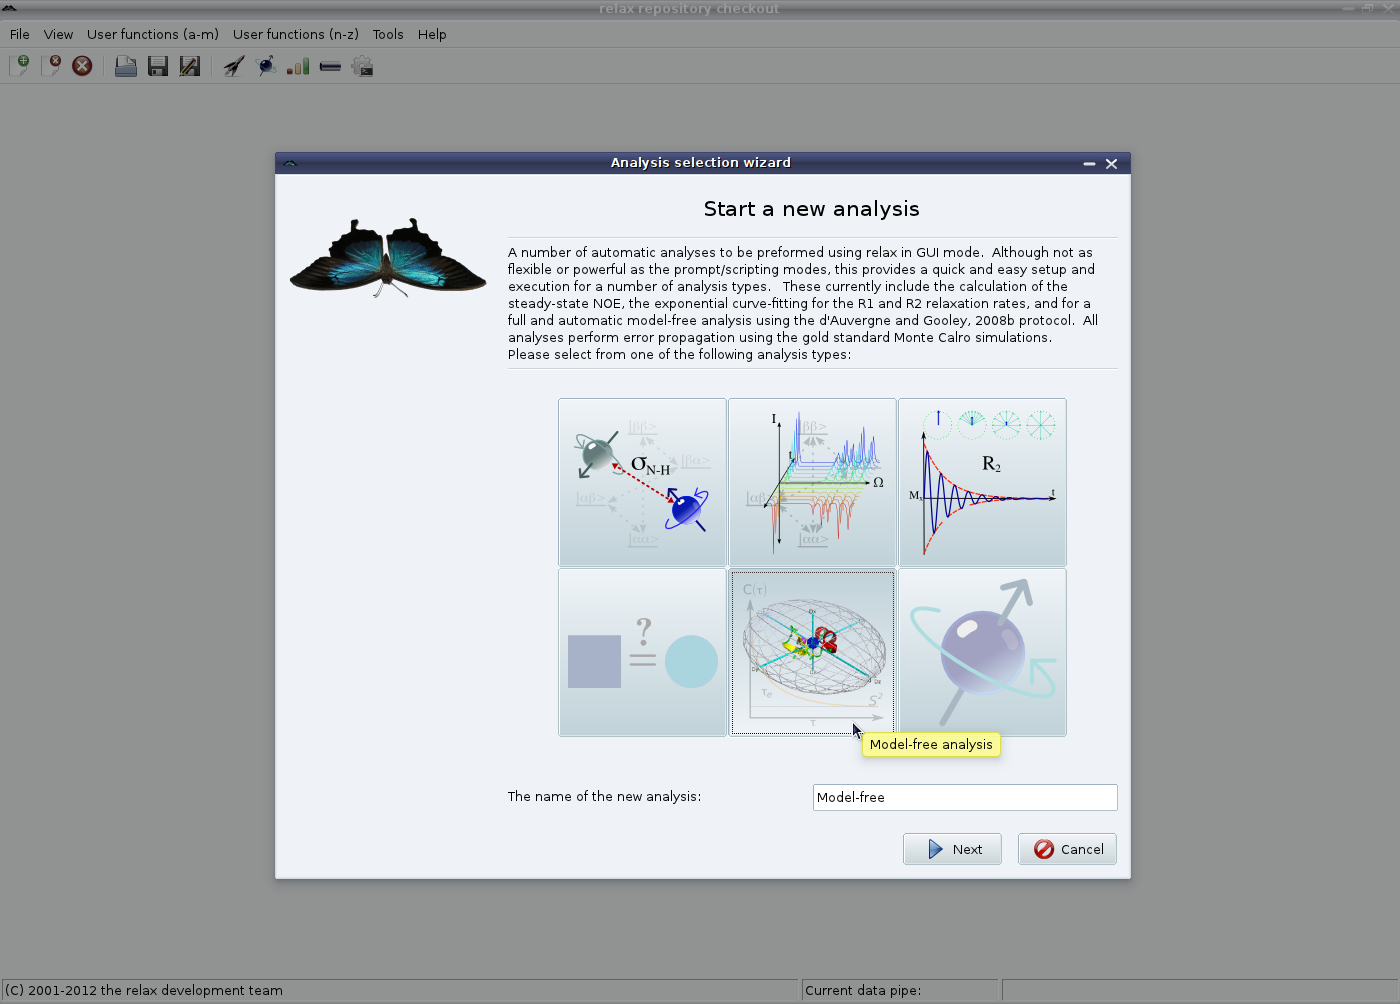
\includegraphics[
      width=0.8\textwidth,
      bb=14 14 1415 1019
    ]
    {graphics/screenshots/mf_analysis/analysis_wizard1}
  }
\end{minipage}

Click on the \guibutton{Next} button and on the second page click on the \guibutton{Start} button.
The text in the second page need not be changed.

\begin{minipage}[h]{\linewidth}
  \centerline{
    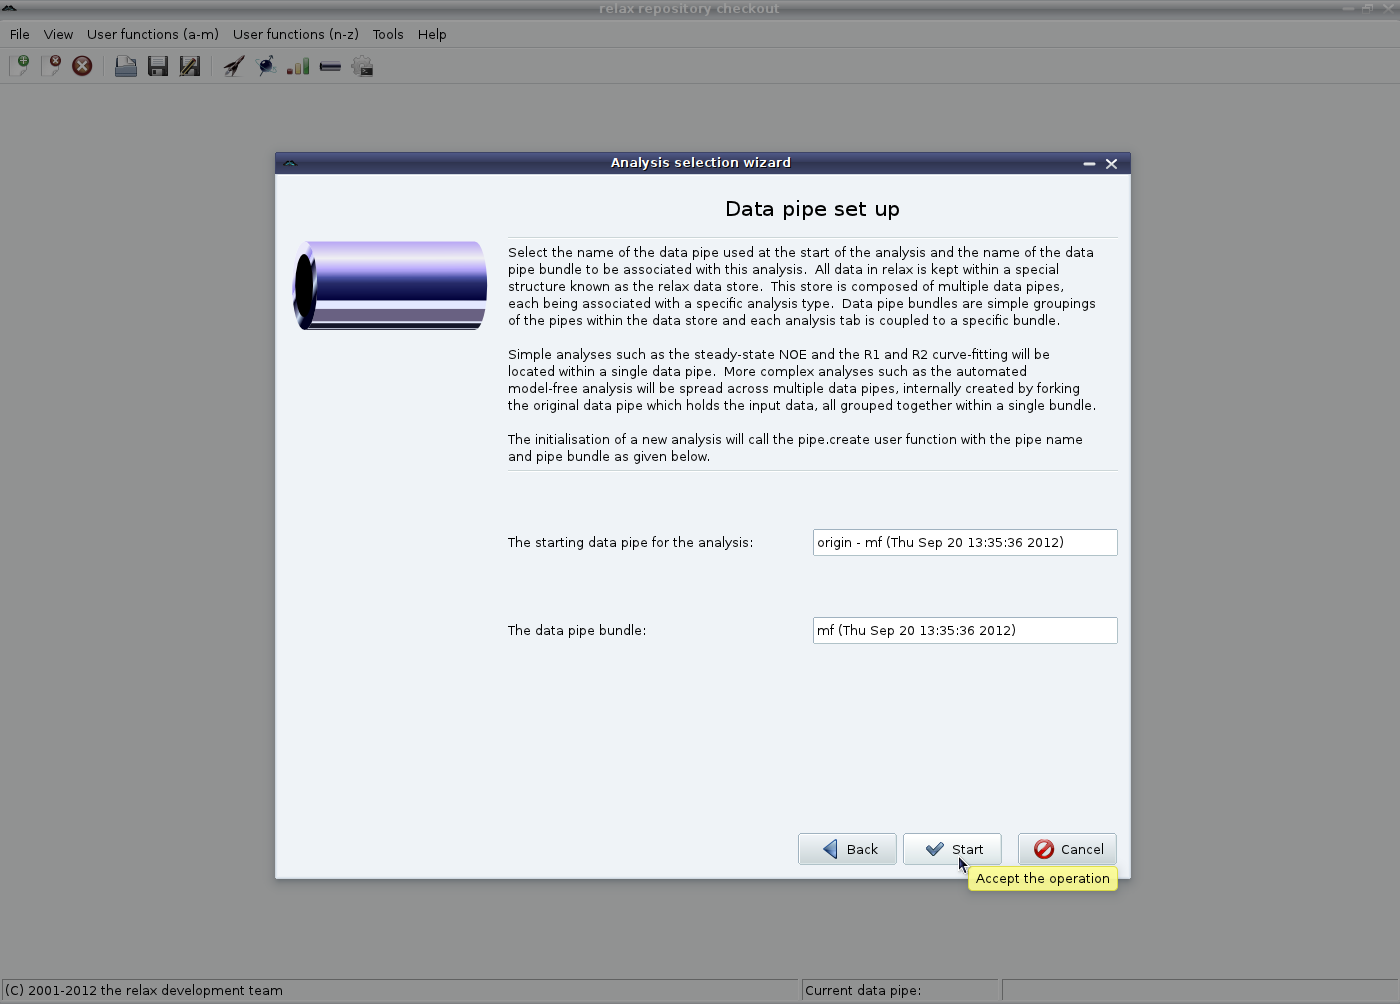
\includegraphics[
      width=0.8\textwidth,
      bb=14 14 1415 1019
    ]
    {graphics/screenshots/mf_analysis/analysis_wizard2}
  }
\end{minipage}


% General setup.
%~~~~~~~~~~~~~~~

\subsection{d'Auvergne protocol GUI mode -- general setup}

Once the analysis is initialised, the screen should look like:

\begin{minipage}[h]{\linewidth}
  \centerline{
    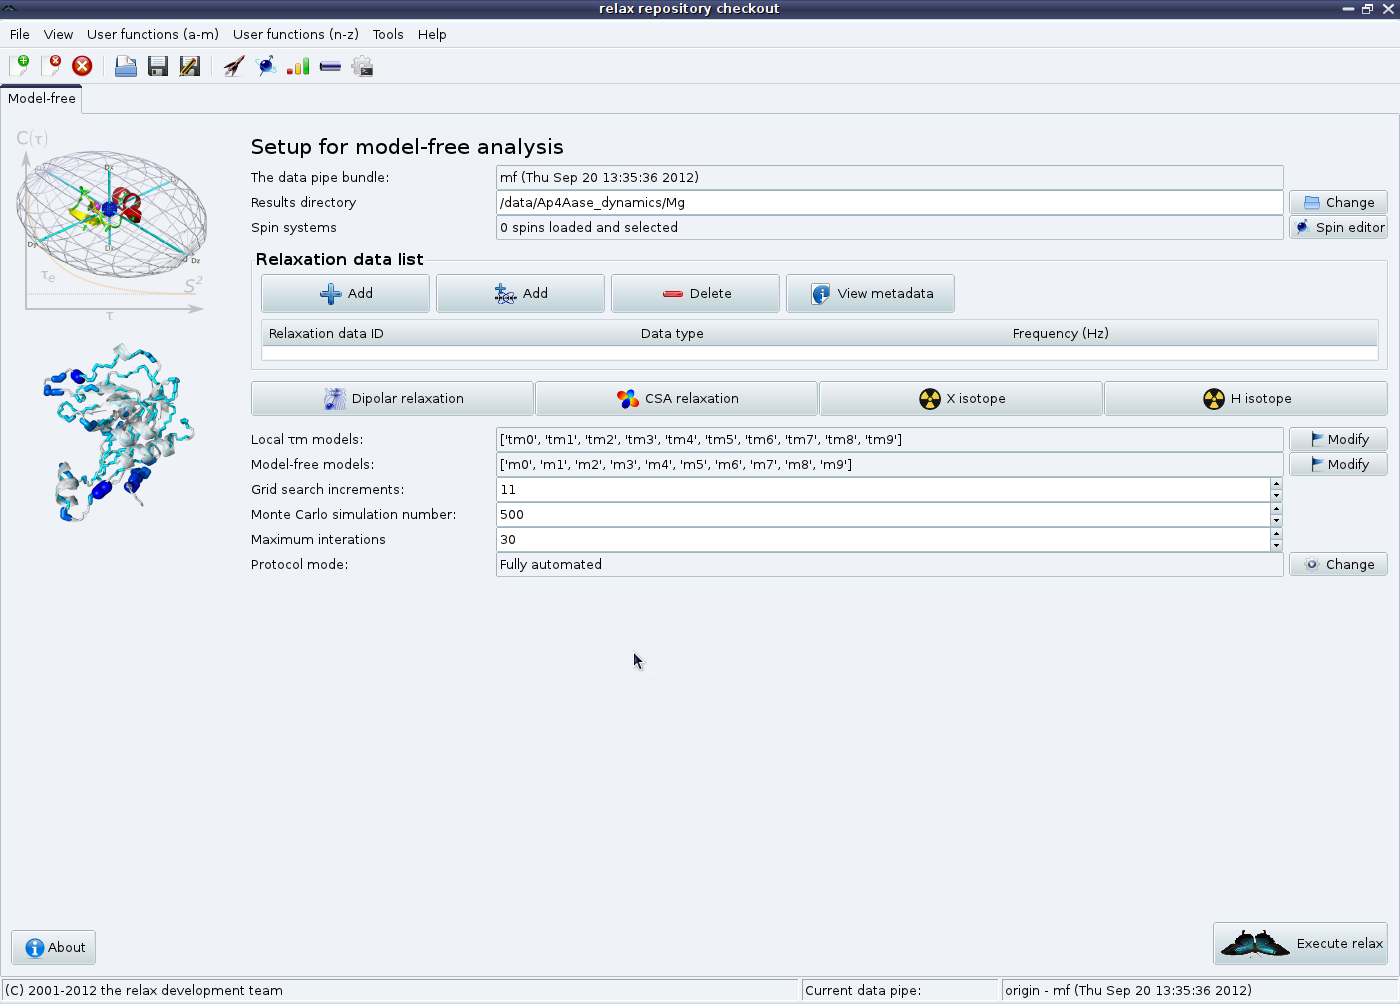
\includegraphics[
      width=0.8\textwidth,
      bb=14 14 1415 1019
    ]
    {graphics/screenshots/mf_analysis/blank}
  }
\end{minipage}

The \guibutton{About} button in the bottom left will bring up a window with the same description as given in the sample script:

\begin{minipage}[h]{\linewidth}
  \centerline{
    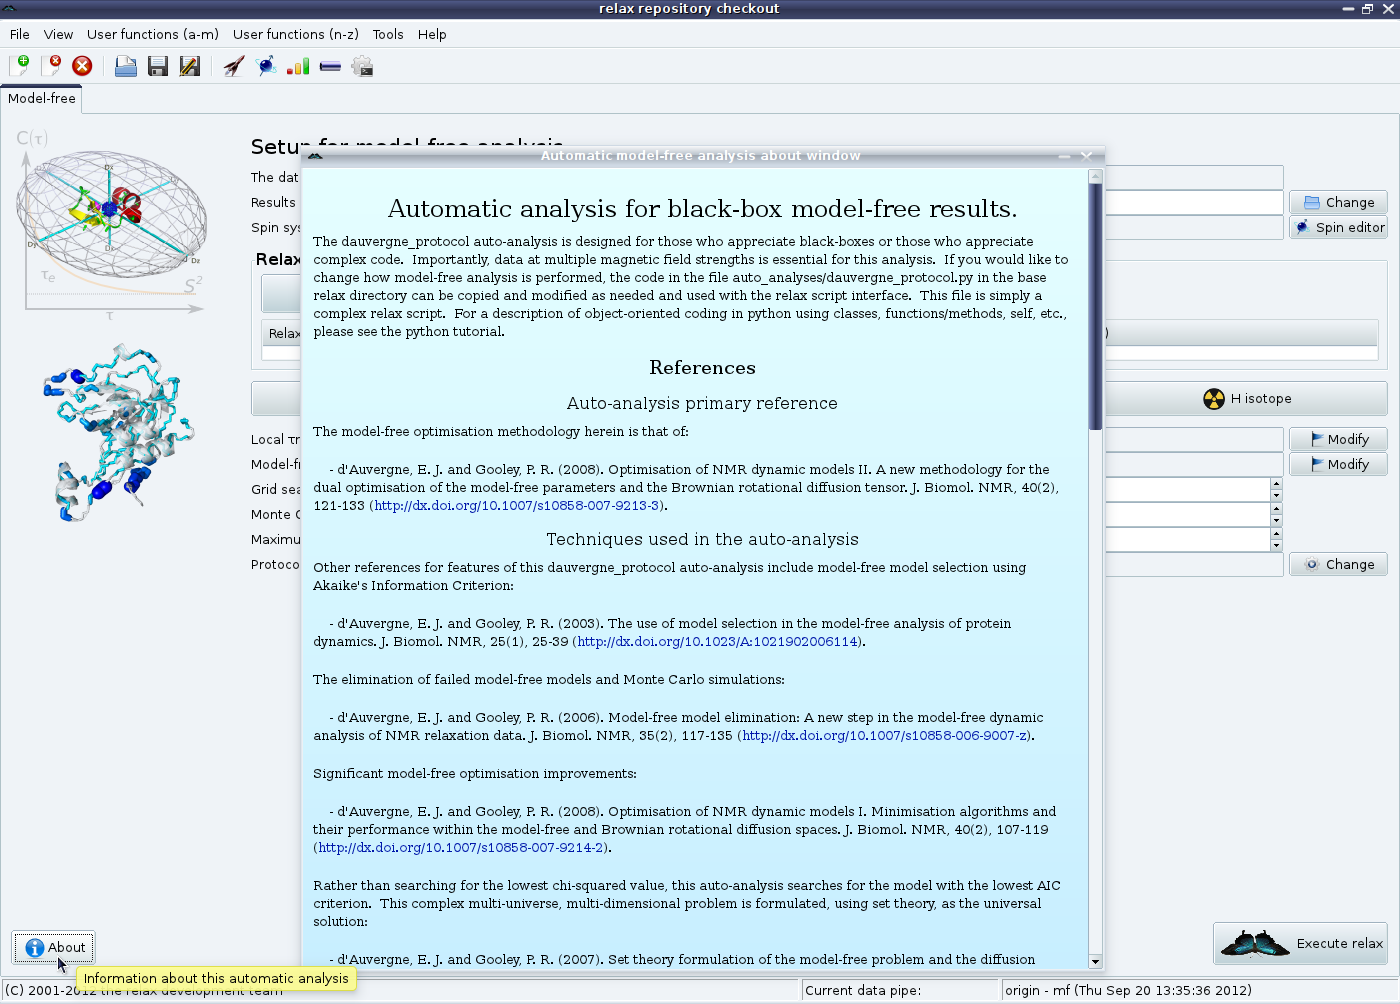
\includegraphics[
      width=0.8\textwidth,
      bb=14 14 1415 1019
    ]
    {graphics/screenshots/mf_analysis/about}
  }
\end{minipage}

At this point, back in the main relax window, the results directory where all of the output files and directories will be saved can be changed.


% Spin systems.
%~~~~~~~~~~~~~~

\subsection{d'Auvergne protocol GUI mode -- setting up the spin systems}

The model-free dynamics is at the level of the spins -- relaxation affects individual nuclei.
In the main model-free tab you will see the \gui{Spin systems} GUI element.
Clicking on the \guibutton{Spin editor} button to the right of this element will launch the spin editor window.

In this tutorial, the \nth{3} model of the PDB file \file{1f3y.pdb} will be used to extract the spin system information.
The molecule will be named \guistring{Ap4Aase}.
For details on how to create the spin containers necessary for this analysis, please see section~\ref{sect: GUI - structural data} on page~\pageref{sect: GUI - structural data} (or analyses lacking structural data in section~\ref{sect: GUI - sequence file} on page~\pageref{sect: GUI - sequence file} for sequence files).

Note that for this tutorial, the protein backbone spins \guistring{@N} and \guistring{@H} as well as the tryptophan sidechain indole \guistring{@NE1} and \guistring{@HE1} spins should be loaded in the spin viewer window.


% Unresolved spins.
%~~~~~~~~~~~~~~~~~~

\subsection{d'Auvergne protocol GUI mode -- unresolved spins}

To deselect all unwanted spins, please read section~\ref{sect: GUI - deselect spins} on page~\pageref{sect: GUI - deselect spins} for all the necessary instructions for how to do this in the GUI.


% Loading the data.
%~~~~~~~~~~~~~~~~~~

\subsection{d'Auvergne protocol GUI mode -- loading the data}

The relaxation data can either come from plain columnar formatted text files (such as if relax was used for the NOE, $\Rone$ and $\Rtwo$ analyses) or from the Bruker Dynamics Centre.
For the former, click on the \guibutton{Add} button in the \gui{Relaxation data list} GUI element.
This route will be used for this tutorial.
For the later, click on the \guibutton{Add Bruker} button.
After clicking on \guibutton{Add}, you will see the relaxation data loading wizard:

\begin{minipage}[h]{\linewidth}
  \centerline{
    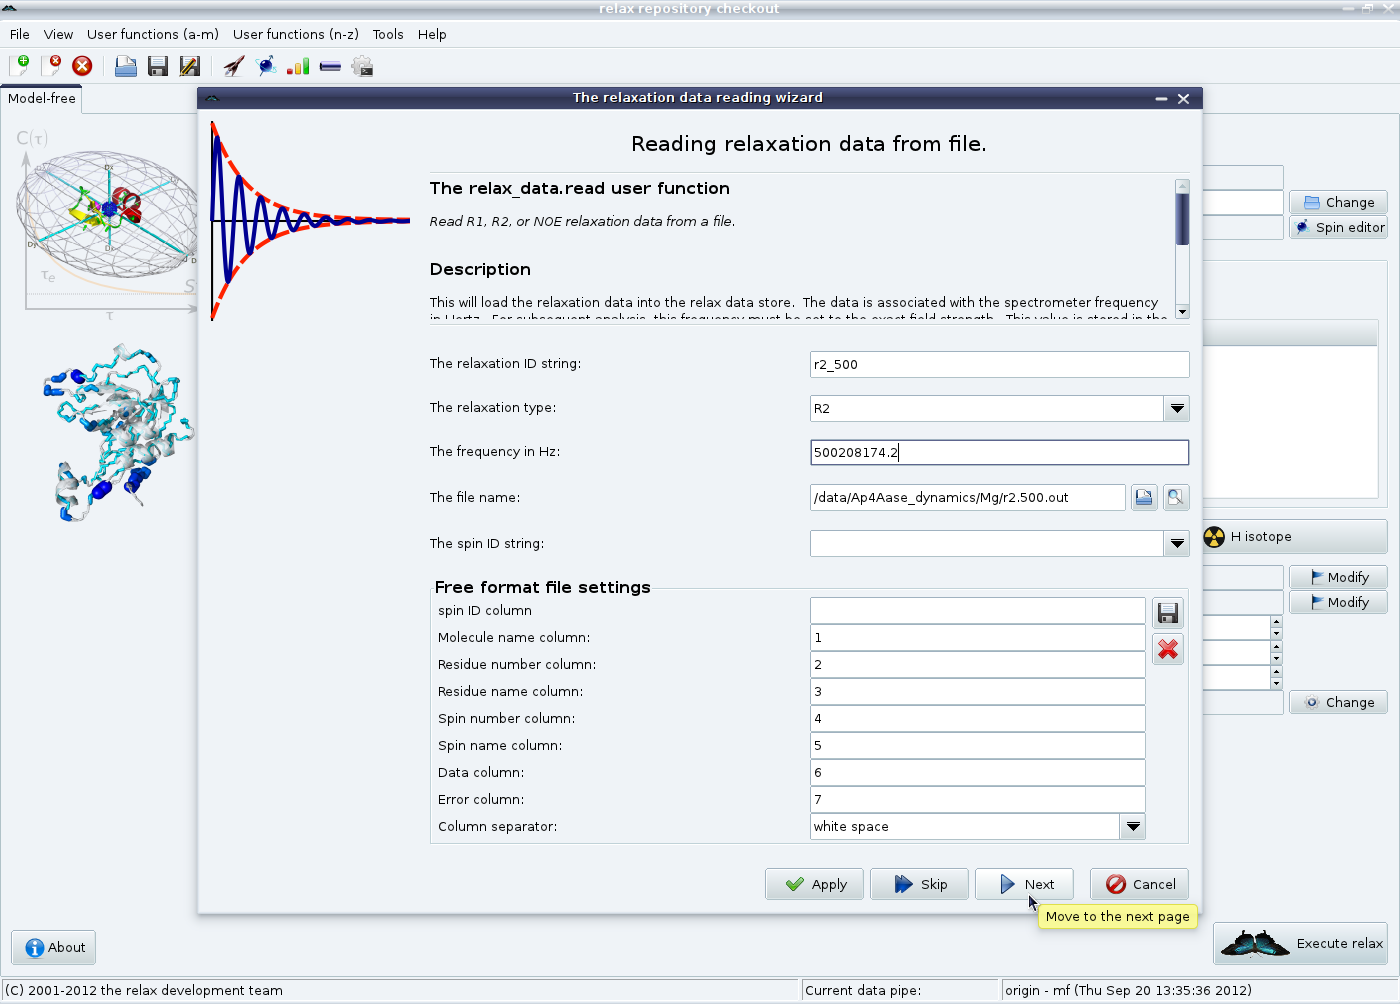
\includegraphics[
      width=0.8\textwidth,
      bb=14 14 1415 1019
    ]
    {graphics/screenshots/mf_analysis/relax_data_file}
  }
\end{minipage}

In this first page, the unique relaxation data identification string (\guistring{r2\_500}), the relaxation data type (\guistring{R2}), the frequency in Hertz (\guistring{500208174.2}) and the file (\guistring{r2.500.out}) are specified.
If your data comes from another program, you many need to change the values in the \gui{Free format file settings} element.
Click on \guibutton{Next} to load the data from the file.

The next wizard pages are for loading the metadata which is used in the BioMagResBank deposition of your final results.
The first is how the peak intensities were measured, either peak heights or volumes.
Select the appropriate value, then click on \guibutton{Next}.

\begin{minipage}[h]{\linewidth}
  \centerline{
    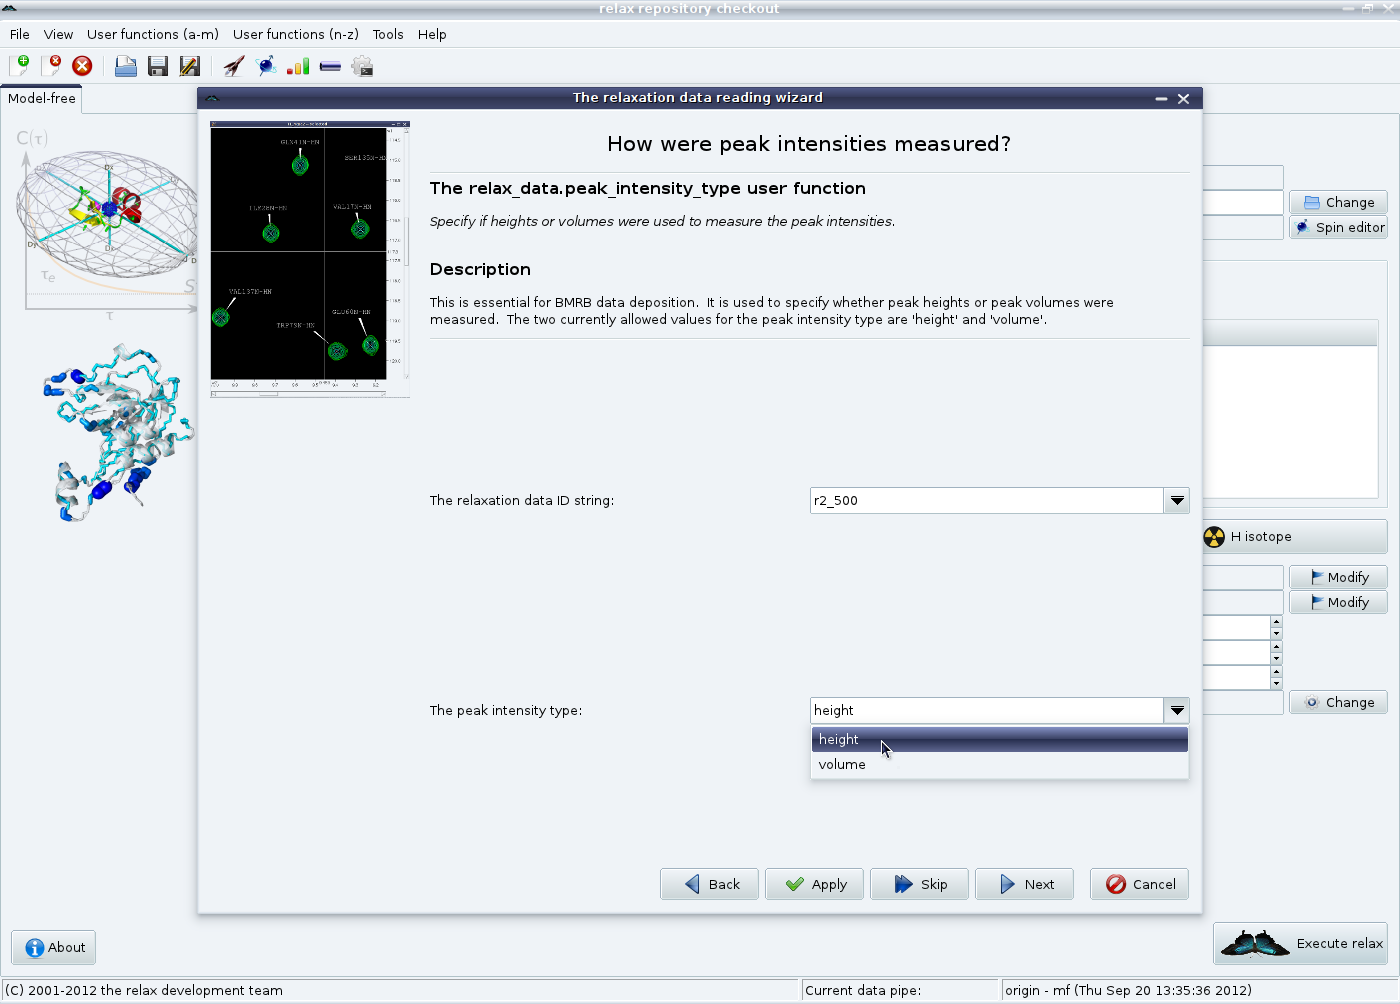
\includegraphics[
      width=0.8\textwidth,
      bb=14 14 1415 1019
    ]
    {graphics/screenshots/mf_analysis/relax_data_intensity}
  }
\end{minipage}

Then the temperature control method is given.
For more details, please read the documentation provided in the wizard and see section~\ref{sect: temperature control and calibration} on page~\pageref{sect: temperature control and calibration}.
Click on \guibutton{Next} to continue.

\begin{minipage}[h]{\linewidth}
  \centerline{
    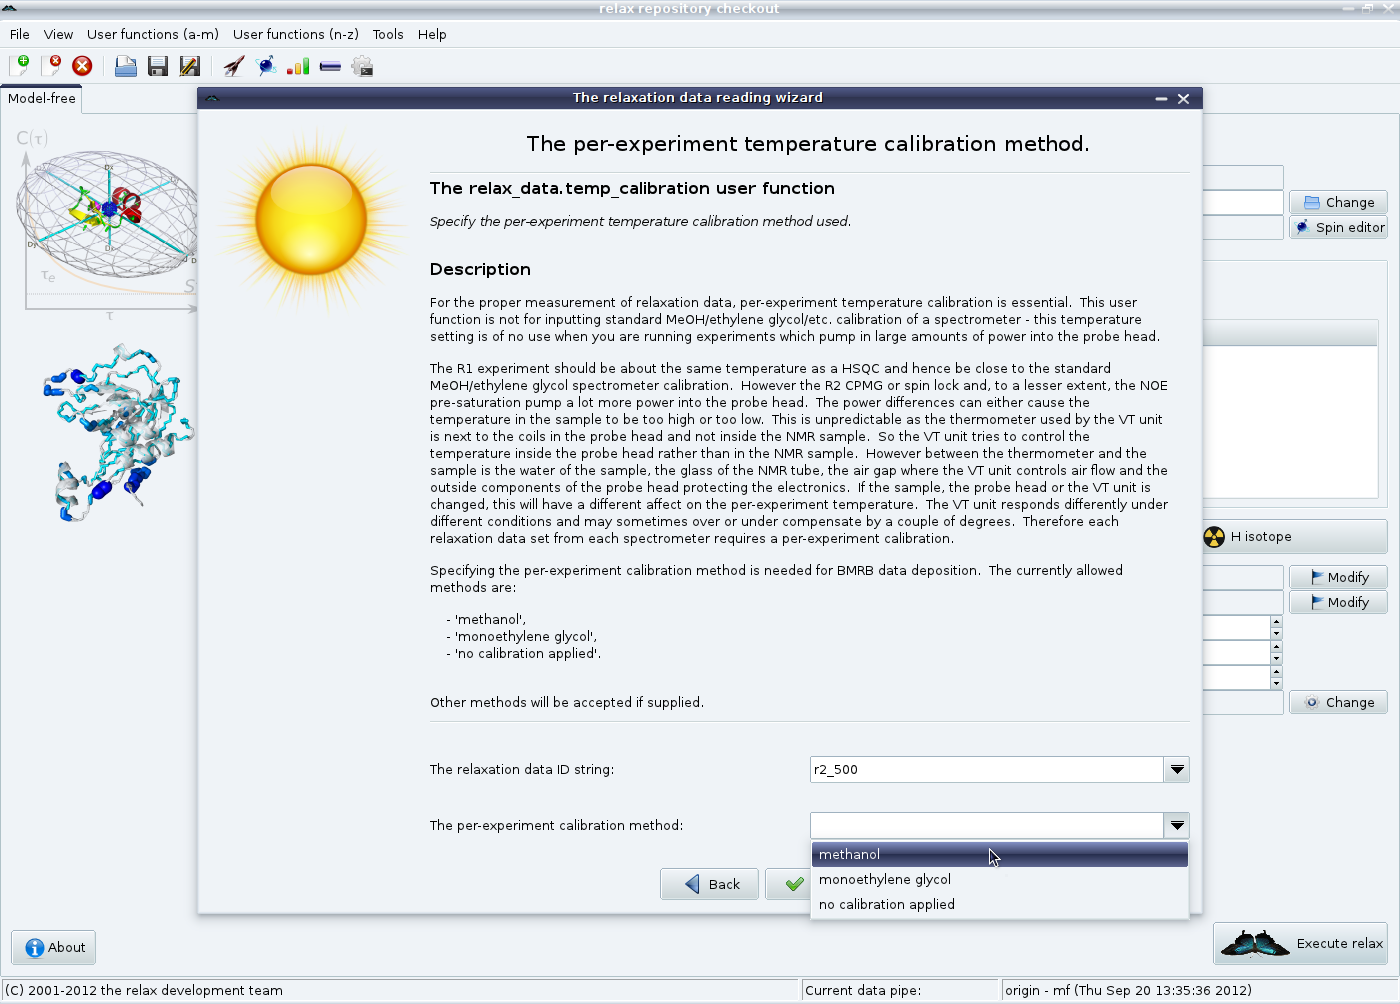
\includegraphics[
      width=0.8\textwidth,
      bb=14 14 1415 1019
    ]
    {graphics/screenshots/mf_analysis/relax_data_temp_control}
  }
\end{minipage}

The temperature calibration method can finally be specified.
Again, see section~\ref{sect: temperature control and calibration} on page~\pageref{sect: temperature control and calibration} for the full details.
Click on the \guibutton{Finish} button to close the wizard.

\begin{minipage}[h]{\linewidth}
  \centerline{
    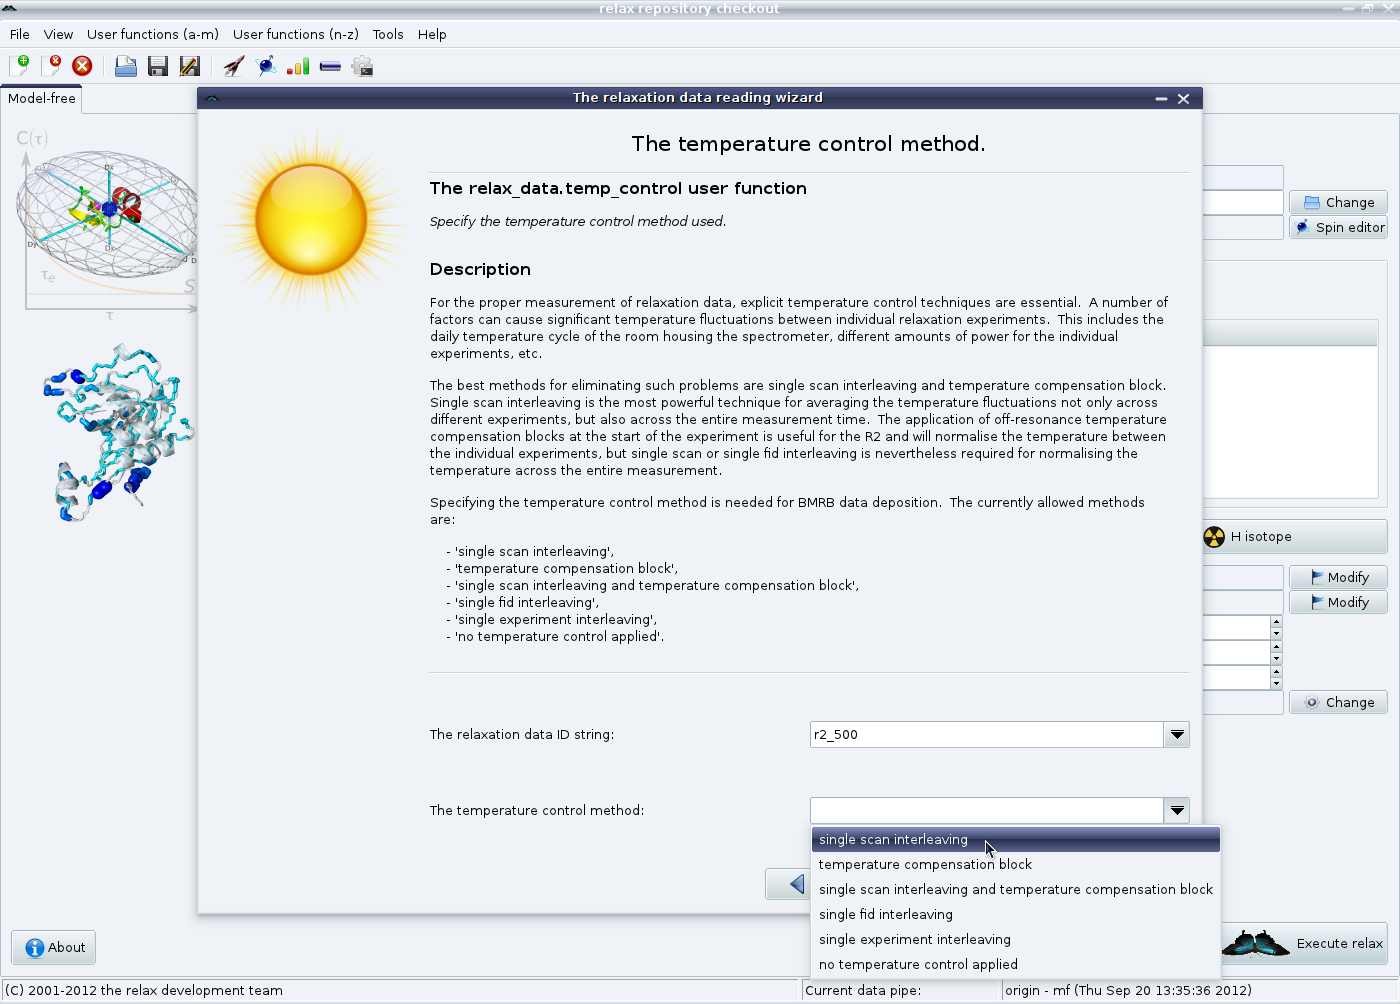
\includegraphics[
      width=0.8\textwidth,
      bb=14 14 1415 1019
    ]
    {graphics/screenshots/mf_analysis/relax_data_temp_calibration}
  }
\end{minipage}

After you have repeated this for the NOE, $\Rone$ and $\Rtwo$ at both 500 and 600 MHz, you should now see:

\begin{minipage}[h]{\linewidth}
  \centerline{
    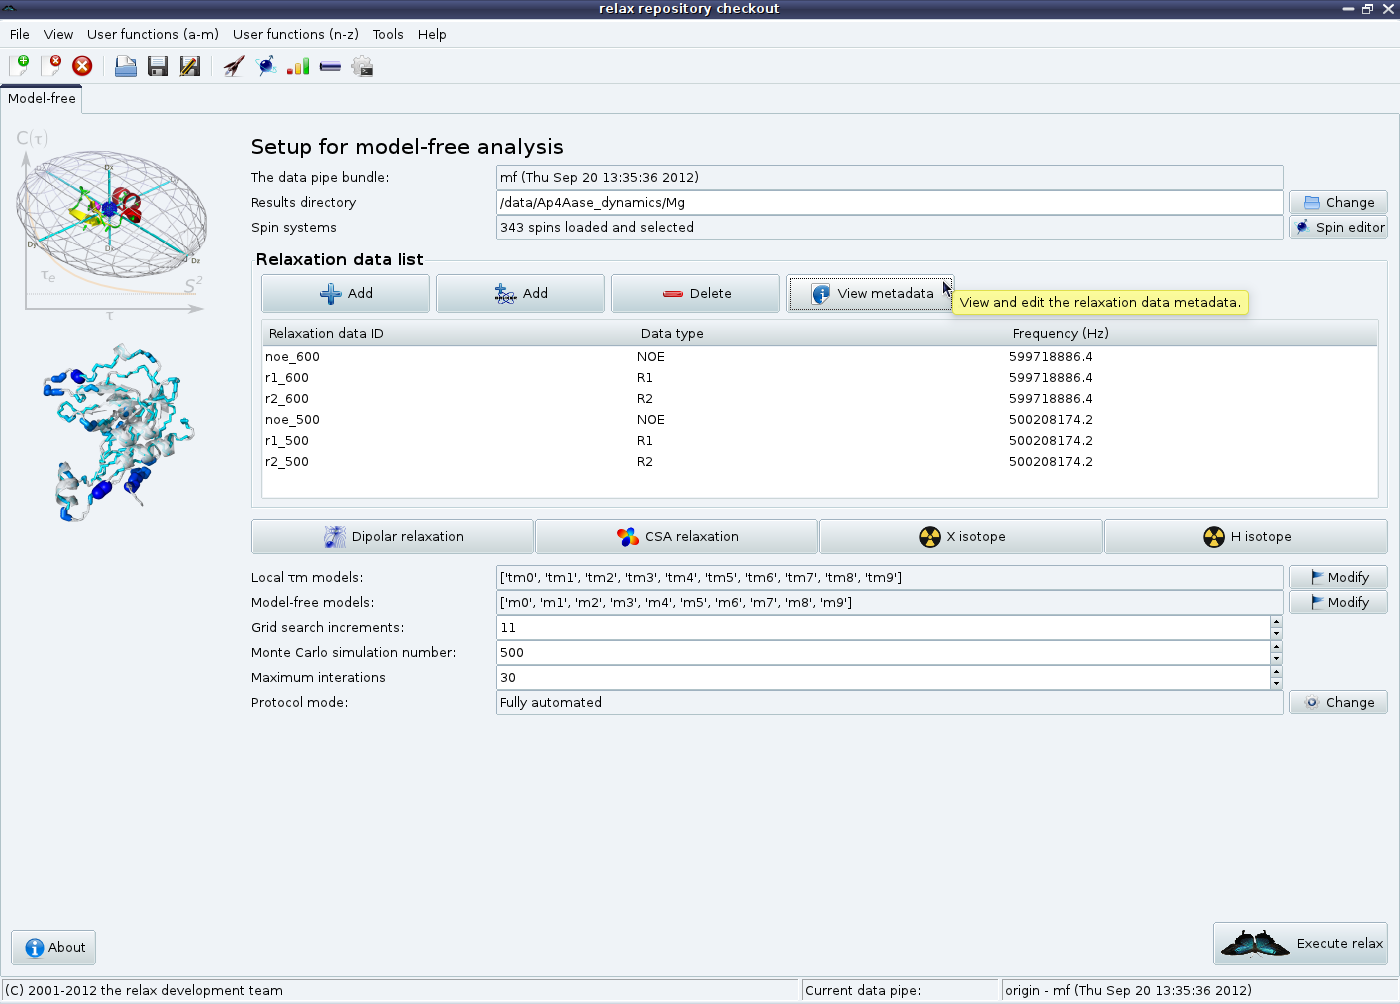
\includegraphics[
      width=0.8\textwidth,
      bb=14 14 1415 1019
    ]
    {graphics/screenshots/mf_analysis/analysis_tab_full}
  }
\end{minipage}

Check that the metadata has been properly entered by clicking on the \guibutton{View metadata} button in the \gui{Relaxation data list} GUI element:

\begin{minipage}[h]{\linewidth}
  \centerline{
    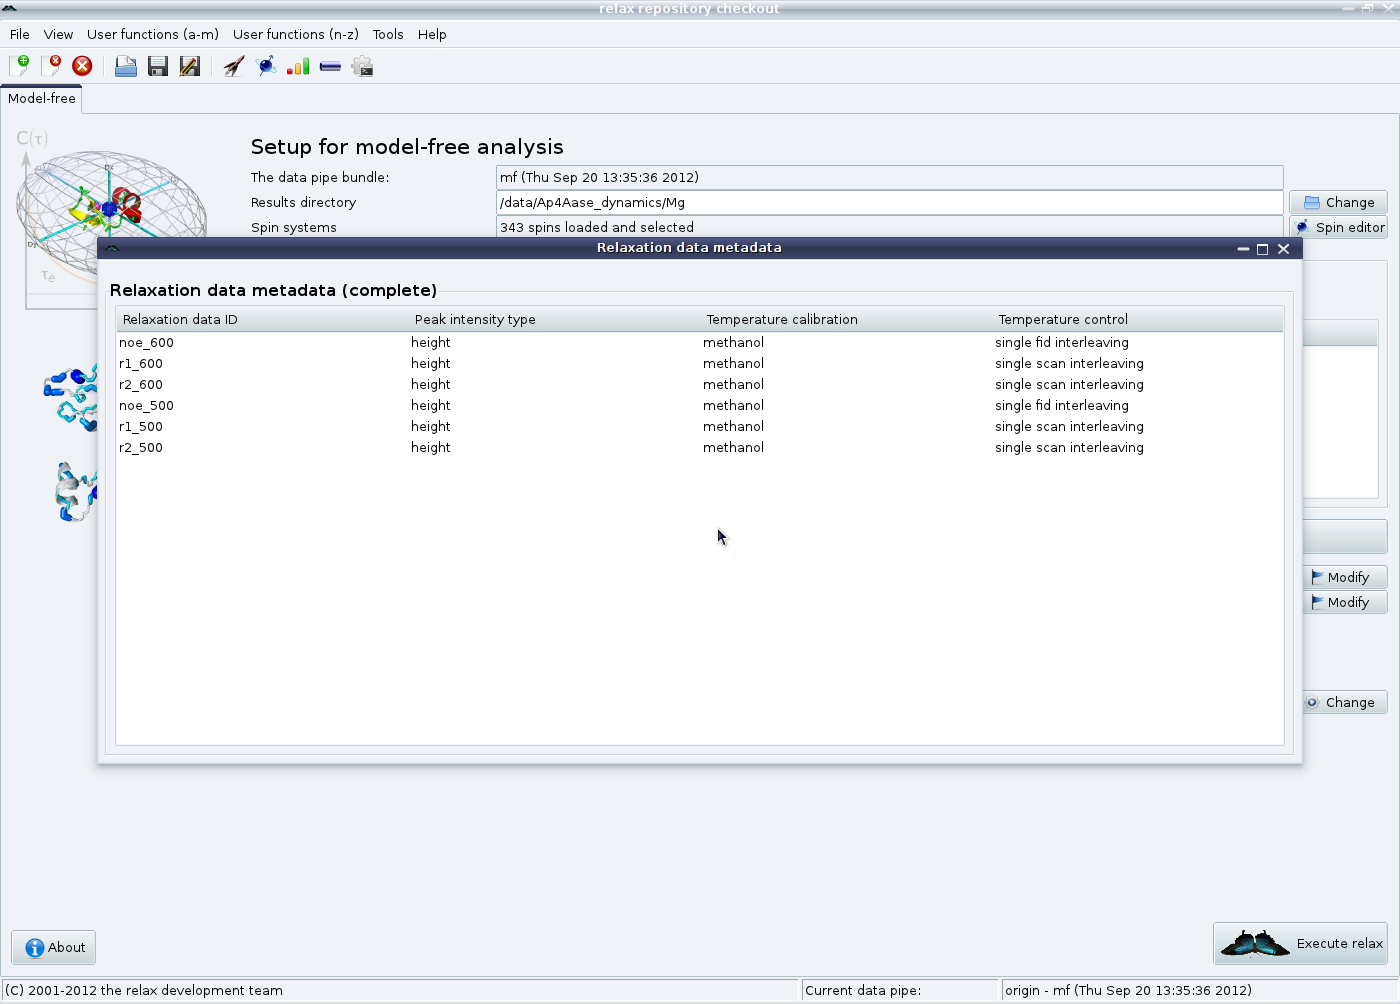
\includegraphics[
      width=0.8\textwidth,
      bb=14 14 1415 1019
    ]
    {graphics/screenshots/mf_analysis/metadata}
  }
\end{minipage}


% The relaxation interactions.
%~~~~~~~~~~~~~~~~~~~~~~~~~~~~~

\subsection{d'Auvergne protocol GUI mode -- relaxation interactions}

Just as in the scripting mode, the relaxation interactions need to now be defined.
The first is the magnetic diole-dipole interaction.
All coupled nitrogen and proton spins should already be loaded at this point.
Click on the \guibutton{Dipolar relaxation} button in the model-free tab in the main relax window to launch the magnetic dipole-dipole interaction wizard:

\begin{minipage}[h]{\linewidth}
  \centerline{
    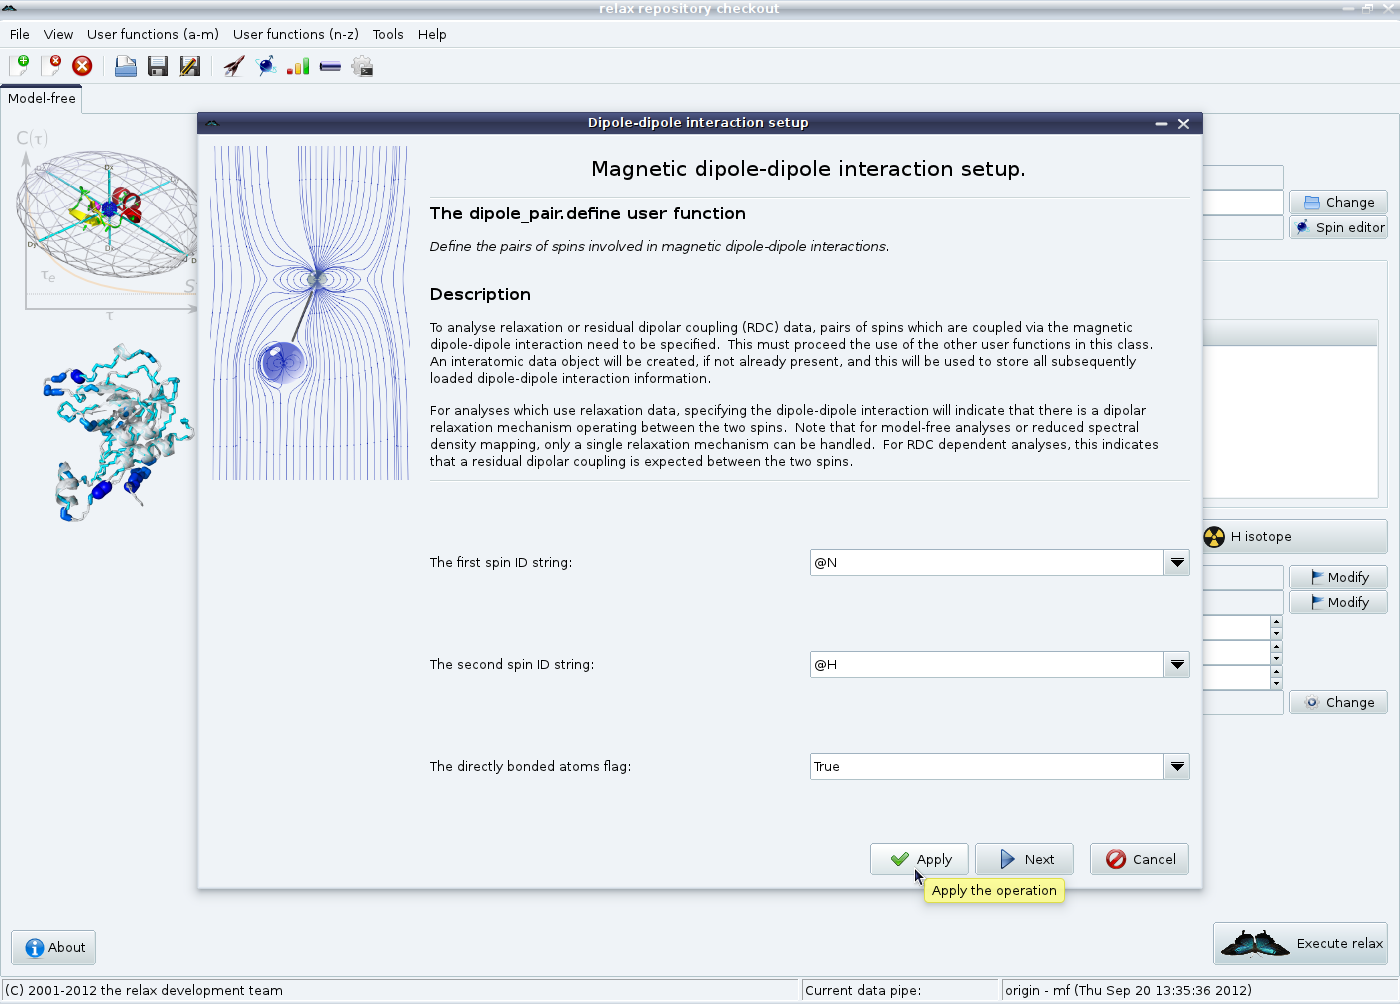
\includegraphics[
      width=0.8\textwidth,
      bb=14 14 1415 1019
    ]
    {graphics/screenshots/mf_analysis/dipole_wizard_define}
  }
\end{minipage}

For this example, directly bonded nitrogens and protons will be analysed.
To start with, the backbone NH pairs will be defined.
Leave the values at \guistring{@N} and \guistring{@H} and click on the \guibutton{Apply} button.
Then change the two spin ID strings to \guistring{@NE1} and \guistring{@HE1} to set up the tryptophan sidechain indole NH pairs and click on the \guibutton{Next} button.
Note that the regular expression \guistring{@N*} and \guistring{@H*} should not be used in this first wizard page as otherwise \prompt{@N} spins will be connected to \prompt{@HE1} spins of the same tryptophan residue and \prompt{@H} spins to \prompt{@NE1} spins.

Now the $\langle r^{-3} \rangle$ averaged distance of 1.02~\AA\ will be set.
Leave all settings as they are and click on \guibutton{Next}:

\begin{minipage}[h]{\linewidth}
  \centerline{
    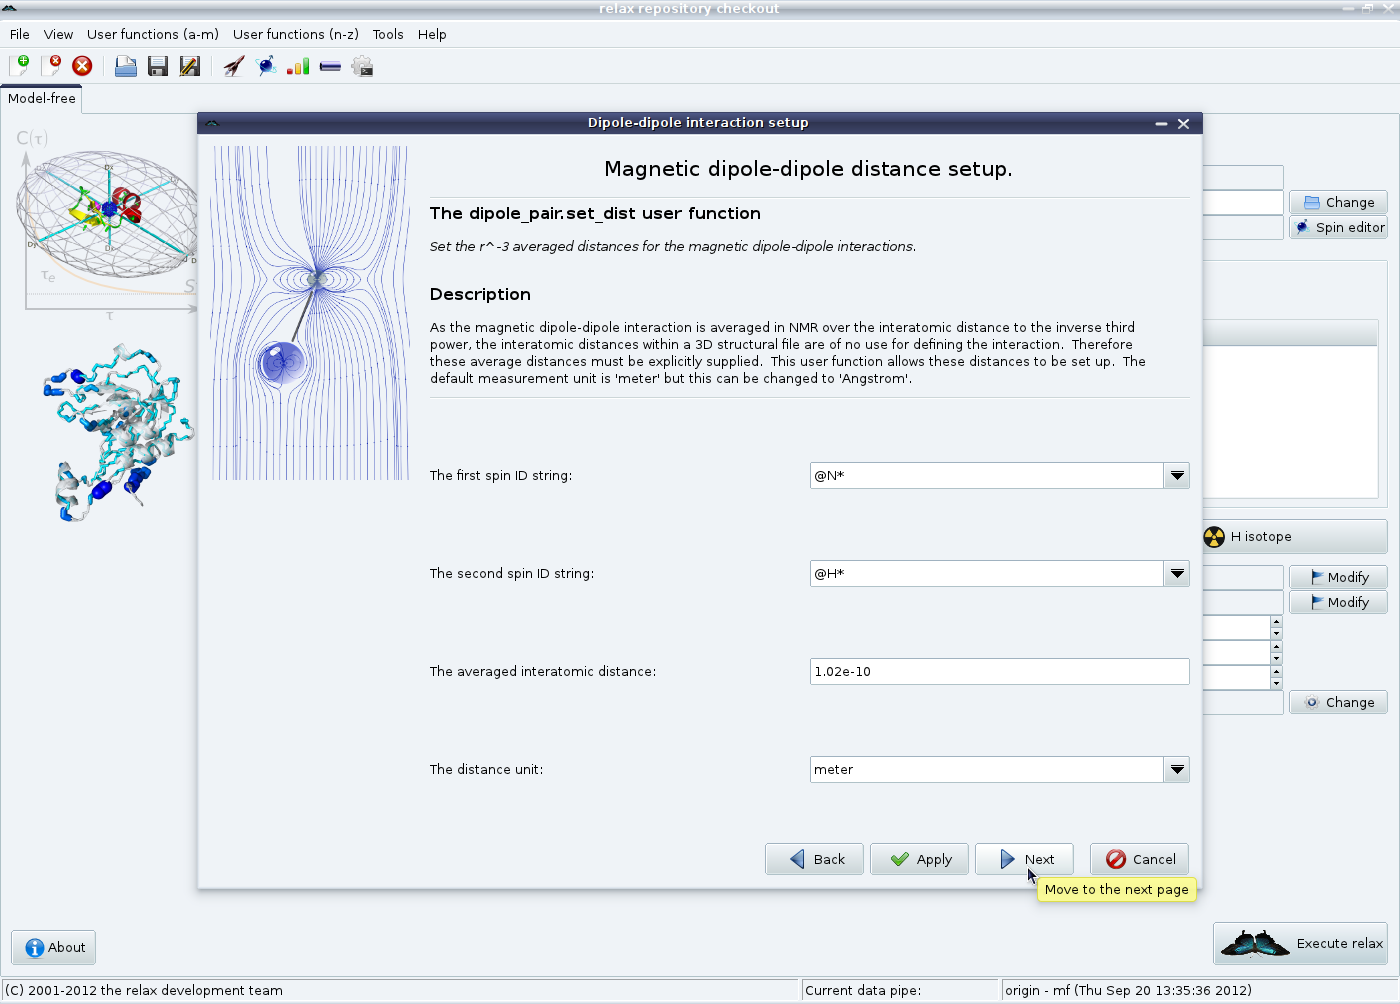
\includegraphics[
      width=0.8\textwidth,
      bb=14 14 1415 1019
    ]
    {graphics/screenshots/mf_analysis/dipole_wizard_distance}
  }
\end{minipage}

If multiple models have been loaded in the previous steps, then the unit vectors between each model need to be calculated.
For a model-free analysis multiple unit vectors must be averaged to a single vector -- current model-free theory is based on the assumption of a single vector orientation.
Therefore the averaged vector flag must be left on \guistring{True}.
Click on \guibutton{Finish} to terminate the set up of the magnetic dipole-dipole interactions:

\begin{minipage}[h]{\linewidth}
  \centerline{
    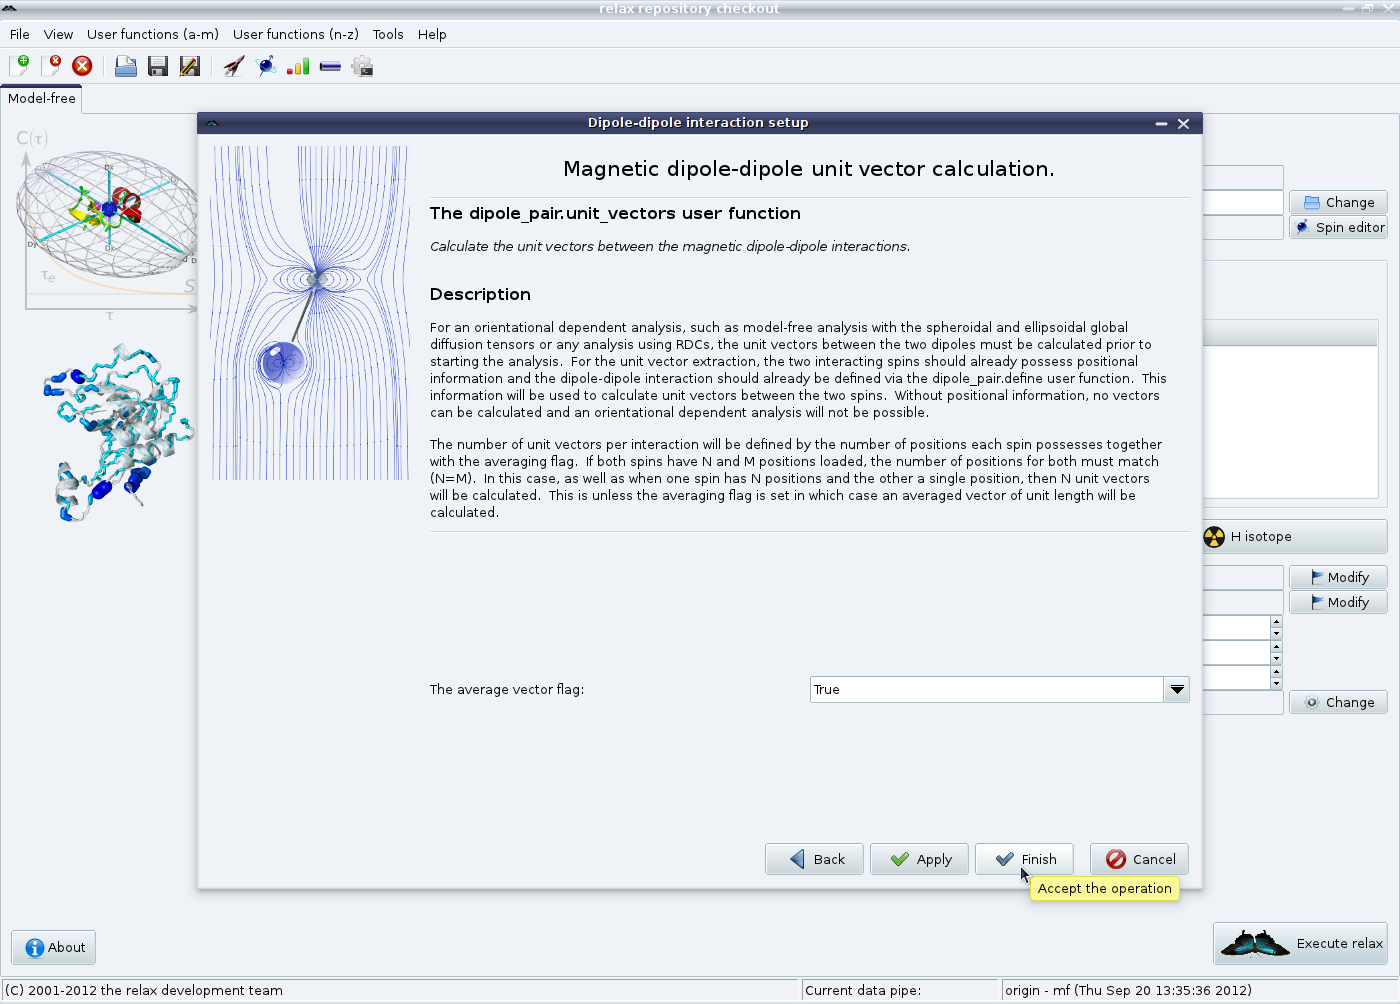
\includegraphics[
      width=0.8\textwidth,
      bb=14 14 1415 1019
    ]
    {graphics/screenshots/mf_analysis/dipole_wizard_unit_vector}
  }
\end{minipage}

Secondly the chemical shift anisotropy (CSA) relaxation mechanism needs to be defined.
Click on the \guibutton{CSA relaxation} button in the model-free tab in the main relax window.
An averaged CSA value of -172~ppm will be used for all spins, so simply click on \guibutton{Ok} to finish.

\begin{minipage}[h]{\linewidth}
  \centerline{
    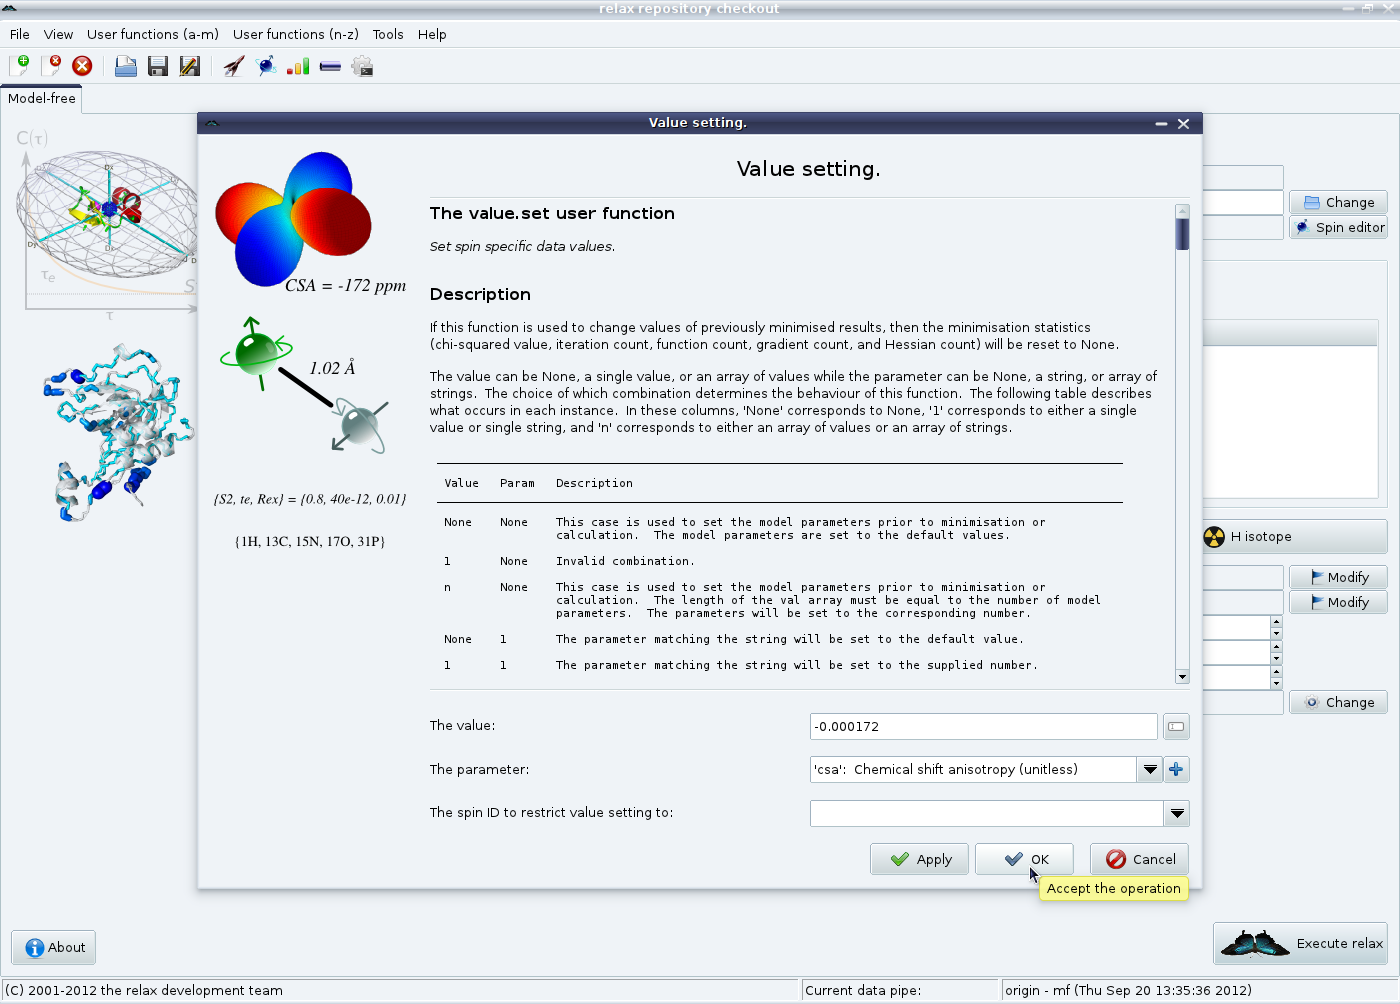
\includegraphics[
      width=0.8\textwidth,
      bb=14 14 1415 1019
    ]
    {graphics/screenshots/mf_analysis/csa_wizard}
  }
\end{minipage}


% The spin isotopes.
%~~~~~~~~~~~~~~~~~~~

\subsection{d'Auvergne protocol GUI mode -- spin isotopes}

As the PDB file contains no isotope information, this needs to now be specified.
First click on the \guibutton{X isotope} button to set the nuclear isotope type of the heteronuclei:

\begin{minipage}[h]{\linewidth}
  \centerline{
    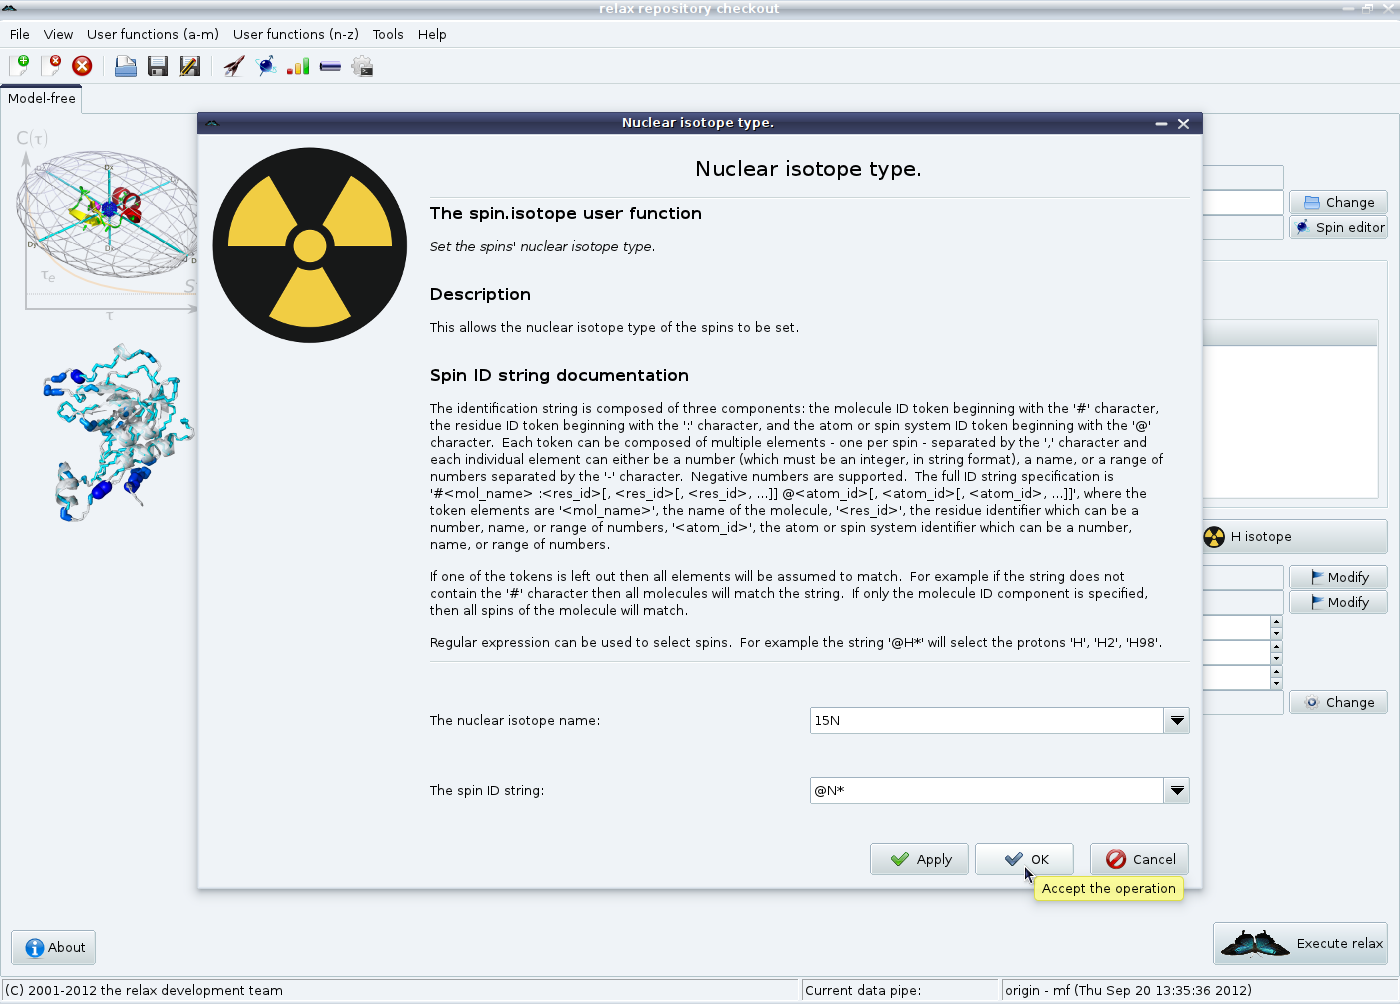
\includegraphics[
      width=0.8\textwidth,
      bb=14 14 1415 1019
    ]
    {graphics/screenshots/mf_analysis/x_isotope}
  }
\end{minipage}

As nitrogen relaxation is being studied, the nuclear isotope name can be left as \guistring{15N} and the spin ID string to \guistring{@N*}.
Therefore simply click on the \guibutton{Ok} button.
Exactly the same procedure can be used for the proton with the \guibutton{H isotope} button.


% The rest of the setup.
%~~~~~~~~~~~~~~~~~~~~~~~
\subsection{d'Auvergne protocol GUI mode -- the rest of the setup}

The local $\tau_m$ models and model-free models should not be modified, the reason for this is explained in section~\ref{sect: d'Auvergne protocol script variables} on page~\pageref{sect: d'Auvergne protocol script variables}.
The grid search increments defaults to \guistring{11}.
This is used in the optimisation of the individual model-free models for each spin.
This value should also not be touched unless you know what you are doing (and have read \citet{dAuvergneGooley08a}).
The number of Monte Carlo simulations can be increased but, for accurate error estimates, it should not be less than 500 simulations.
One additional setting is the \gui{Maximum iterations}.
This is a maximum number of times the protocol will iterate before terminating.
This allows infinite loops to be broken.
The value of 30 iterations should be fine for most analyses.

The \gui{Protocol mode} GUI element setting of \gui{Fully automated} will not be changed for the analysis of this tutorial.
However if you are studying a system without a 3D structure, you can execute each individual component of the analysis by clicking on the \guibutton{Change} button.
This will make the protocol mode selection window appear:

\begin{minipage}[h]{\linewidth}
  \centerline{
    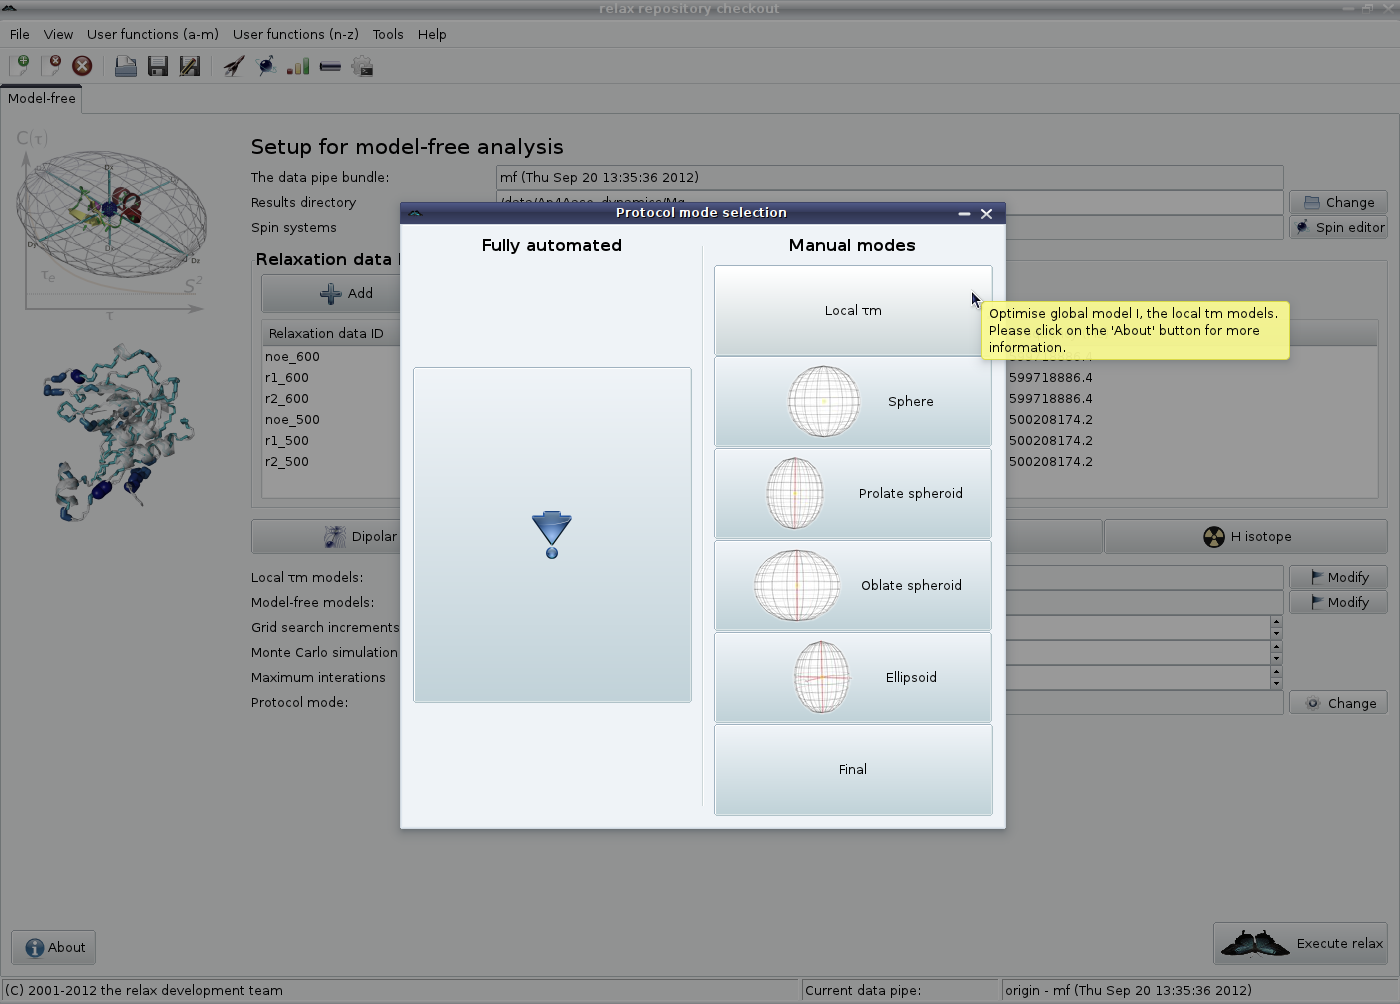
\includegraphics[
      width=0.8\textwidth,
      bb=14 14 1415 1019
    ]
    {graphics/screenshots/mf_analysis/protocol_mode}
  }
\end{minipage}

From this you can first select the \gui{Local $\tau$m} model, then the \gui{Sphere} and finally the \gui{Final} mode, clicking on \guibutton{Execute relax} between each selection.


% Execution.
%~~~~~~~~~~~
\subsection{d'Auvergne protocol GUI mode -- execution}

Prior to executing relax, you should very carefully check the relax controller window for any strange messages, warnings or errors.
You can open this window in three ways:
\begin{itemize}
  \item Selecting the \guimenuitemtwo{View}{Controller} menu item.
  \item Typing \shortcutkey{Ctrl+Z} within the main relax window.
  \item Clicking on the \guibutton{relax controller} button on the toolbar.
\end{itemize}

These messages are very important and will indicate to you if there are any problems prior to starting the very long model-free calculation.
This information should be stored in the \file{log} file as well.
As the execution of a fully iterative and complete model-free protocol takes a very long time to finish, it is advisable to save the current relax state.
This will allow you restart the calculation without performing all of the steps detailed above.
Just in case you cannot work out how to do this yourself, here is a list of the different ways you can do this (if this is not enough for you, please email the relax-users mailing list with your suggestions):
\begin{itemize}
  \item Selecting the \guimenuitemtwo{File}{Save relax state} menu item.
  \item Typing \shortcutkey{Ctrl+S} within the main relax window.
  \item Clicking on the \guibutton{Save relax state} button on the toolbar.
  \item Selecting the \guimenuitemtwo{File}{Save as...} menu item.
  \item Typing \shortcutkey{Shift+Ctrl+S} within the main relax window.
  \item Clicking on the \guibutton{Save as} button on the toolbar.
  \item Selecting the \guimenuitemthree{User functions}{state}{save} menu item.
  \item Opening up the relax prompt window with \guimenuitemtwo{View}{relax prompt} or \shortcutkey{Ctrl+P} and using the \uf{state\ufsep{}save} user function.
\end{itemize}

If all the messages in the relax controller or \file{log} file appear to be fine and you have saved the current relax state, then click on \guibutton{Execute relax}.
This will start the calculations, freeze most of the GUI and open up the relax controller to give you feedback on the progress of the calculations:

\begin{minipage}[h]{\linewidth}
  \centerline{
    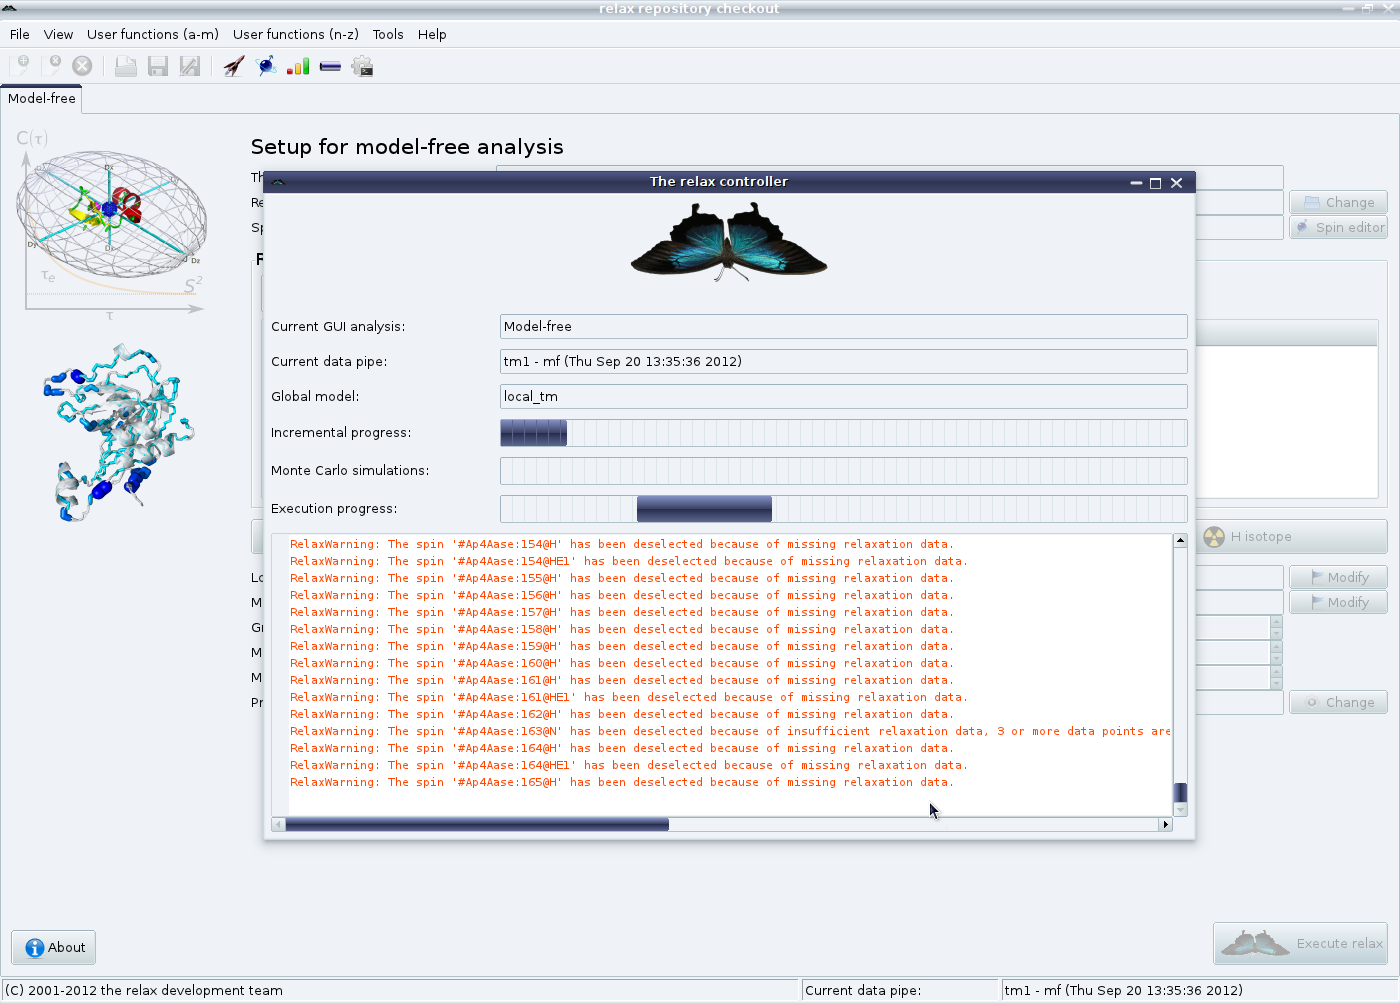
\includegraphics[
      width=0.8\textwidth,
      bb=14 14 1415 1019
    ]
    {graphics/screenshots/mf_analysis/relax_controller_executing}
  }
\end{minipage}

At the start of the protocol, you should again check the messages carefully to be sure that relax is operating as you would expect.
There may be very important \prompt{RelaxWarnings} that will require you to quit relax and start the analysis all over again.


% Completion.
%~~~~~~~~~~~~
\subsection{d'Auvergne protocol GUI mode -- completion}

Upon completion of the analysis, the save and results files for the final result will be located in the \directory{final} directory within the selected results directory.
The results files will consist of text files for each of the spin specific model-free parameters, 2D Grace plots of the model-free parameters, PyMOL and MOLMOL macros for superimposing the model-free parameter values onto the 3D structure of the molecule, and a PDB representation of the final diffusion tensor.

Further visualisations of the results are possible via the \guimenuitemone{User functions} menu entry.
For example to generate a 2D plot of order parameters for one of the other diffusion tensor results, the pipe editor window can be used to switch data pipes to the other diffusion models and then the \guimenuitemthree{User functions}{grace}{write} menu item can be selected to create the plot.


% BMRB.
%~~~~~~
\subsection{d'Auvergne protocol GUI mode -- BMRB deposition}

Once you are ready to publish your results, the very last step of the model-free analysis is to create a NMR-STAR formatted file for \href{http://www.bmrb.wisc.edu/}{BioMagResBank} submission for each model-free analysis you perform.
This can be accomplished using the BMRB export window.
Simply select the \guimenuitemtwo{File}{Export for BMRB deposition} menu item.
You will then see the BMRB export window:

\begin{minipage}[h]{\linewidth}
  \centerline{
    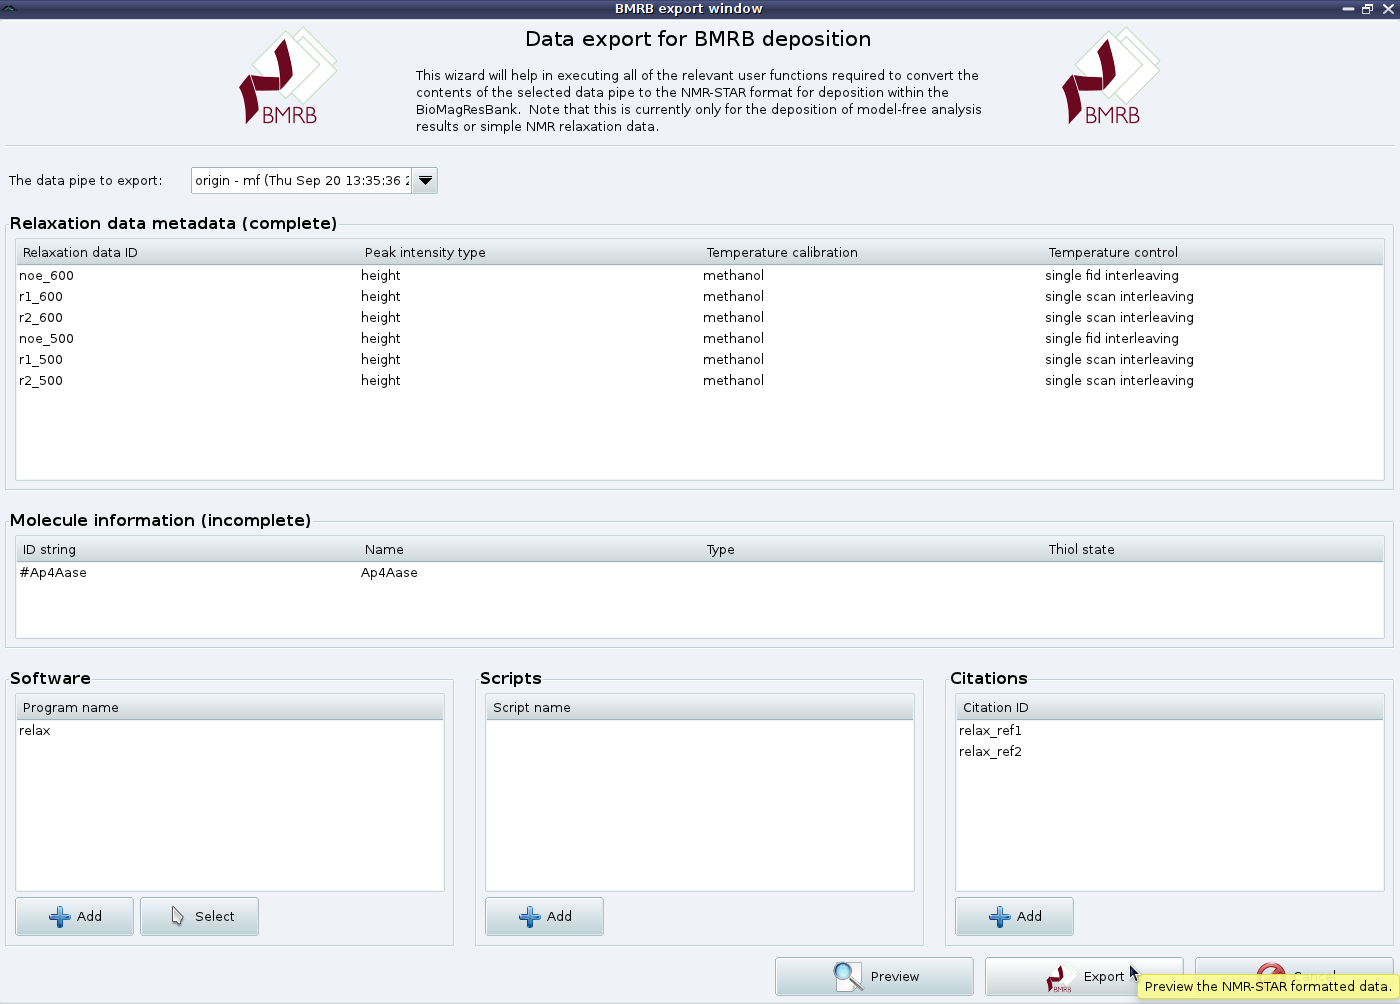
\includegraphics[
      width=0.8\textwidth,
      bb=14 14 1415 1019
    ]
    {graphics/screenshots/mf_analysis/bmrb_export_window}
  }
\end{minipage}

From here you can complete the relaxation data metadata if needed, set up all the molecule information needed for a BMRB deposition, specify the software you have used running up to the model-free analysis and any spectral processing or relax scripts you have used.
You can also add as many citations relevant to your analysis as you wish.
The NMR-STAR formatted file can be previewed in the relax controller window via the \guibutton{Preview} button and the final file created using the \guibutton{Export} button.

Once you are in the stage of writing up, simply go to the ADIT-NMR webpage at \href{http://deposit.bmrb.wisc.edu/bmrb-adit/}{http://deposit.bmrb.wisc.edu/bmrb-adit/},  create a new BMRB deposition, upload the file you have created, complete the deposition as needed, and add the BMRB deposition number to your paper.
